\chapter{Base de datos y diccionario de datos}
\label{anx:base_datos}

Este anexo documenta de forma completa la base de datos de la plataforma, descrita en forma resumida en la Sección~\ref{sec:bd}. Se presentan la organización general del esquema, los diagramas entidad-relación de cada módulo y el diccionario de datos de las 29 tablas que lo conforman.

\section{Organización del esquema}
La información operativa se almacena en una base de datos PostgreSQL 16 (\texttt{defensoria\_db}). Las tablas no se crean mediante guiones manuales: cada microservicio declara sus entidades con la especificación de persistencia de Java y el mapeador objeto-relacional las crea o actualiza al arrancar. Por ello, el esquema que aquí se documenta se obtuvo directamente de las entidades del código fuente de los microservicios.

Cada tabla tiene un microservicio responsable de su escritura. Algunas tablas, como \texttt{quejas} o \texttt{personal\_administrativo}, son consultadas por varios servicios mediante entidades independientes que apuntan a la misma tabla física. Las relaciones entre tablas de servicios distintos no se declaran como llaves foráneas, sino como \emph{referencias lógicas}: el registro hijo guarda el folio o el identificador del registro padre y la integridad se verifica en la lógica del servicio. Esta decisión mantiene independientes los microservicios, a cambio de que la base de datos no impida por sí sola una referencia inválida entre módulos. Algunas referencias lógicas utilizan el correo electrónico en lugar de un identificador; es el caso de las notificaciones, la bitácora de acciones y las plantillas, que guardan el correo del destinatario o de la persona del personal que realizó la acción. La tabla \texttt{preguntas\_chatbot} es la única que no se relaciona con ninguna otra.

En los diagramas y en el diccionario se emplea la siguiente notación:

\begin{itemize}
	\item \textbf{PK:} llave primaria.
	\item \textbf{FK:} llave foránea declarada en la base de datos (línea continua en los diagramas).
	\item \textbf{RL:} referencia lógica a otra tabla, sin llave foránea declarada (línea discontinua en los diagramas).
	\item \textbf{U:} restricción de unicidad.
	\item \textbf{Nulo:} indica si la columna admite valores nulos.
\end{itemize}

La Tabla~\ref{tab:anx_tablas} resume las tablas por módulo y su microservicio responsable.

\rowcolors{2}{rowblue}{white}
\small
\renewcommand{\arraystretch}{1.2}
\setlength{\tabcolsep}{4pt}
\begin{longtable}{|L{4.6cm}|L{3.6cm}|L{7.4cm}|}
	\hiderowcolors\caption{Tablas de la base de datos por módulo}
	\label{tab:anx_tablas} \\ \showrowcolors
	\hline
	\rowcolor{headerblue}
	\headercell{Tabla} & \headercell{Servicios} & \headercell{Contenido} \\
	\hline
	\endfirsthead
	\hline
	\rowcolor{headerblue}
	\headercell{Tabla} & \headercell{Servicios} & \headercell{Contenido} \\
	\hline
	\endhead

	\multicolumn{3}{|l|}{\cellcolor{white}\textbf{Núcleo de quejas}} \\ \hline
	\texttt{acuerdos\_\allowbreak{}conciliacion} & revision-\allowbreak{}service, queja-\allowbreak{}service, primer-\allowbreak{}contacto-\allowbreak{}service & Acuerdos de conciliación propuestos por la Defensoría y la respuesta del quejoso. \\ \hline
	\texttt{notificaciones} & notificaciones-\allowbreak{}service & Avisos persistidos para cada destinatario, con su estado de lectura. \\ \hline
	\texttt{queja\_\allowbreak{}evidencias} & queja-\allowbreak{}service & Archivos de evidencia adjuntos a una queja, almacenados con su contenido binario. \\ \hline
	\texttt{queja\_\allowbreak{}tutores} & queja-\allowbreak{}service & Datos del tutor o adulto responsable cuando el quejoso es menor de edad; relación uno a uno con la queja. \\ \hline
	\texttt{quejas} & queja-\allowbreak{}service, revision-\allowbreak{}service, primer-\allowbreak{}contacto-\allowbreak{}service, subdefensoria-\allowbreak{}service & Registro central de cada queja: folio, identidad del quejoso, narrativa de los hechos, persona señalada, estatus y datos del flujo de recepción (validación, rechazo y turnado). Es la tabla de la que parte todo el expediente. \\ \hline
	\texttt{usuarios} & auth-\allowbreak{}service, queja-\allowbreak{}service & Cuentas de seguimiento de los quejosos: identidad institucional, credencial cifrada, datos de contacto y código de recuperación. \\ \hline
	\multicolumn{3}{|l|}{\cellcolor{white}\textbf{Primer Contacto}} \\ \hline
	\texttt{antecedentes\_\allowbreak{}primer\_\allowbreak{}contacto} & primer-\allowbreak{}contacto-\allowbreak{}service & Antecedentes vinculados a un expediente, ya sea sugeridos por el modelo de búsqueda o agregados manualmente, con la decisión del analista. \\ \hline
	\texttt{citas\_\allowbreak{}primer\_\allowbreak{}contacto} & primer-\allowbreak{}contacto-\allowbreak{}service & Citas programadas con el quejoso o con la persona señalada durante el análisis, con su estado y la respuesta de la persona citada. \\ \hline
	\texttt{dictamenes\_\allowbreak{}primer\_\allowbreak{}contacto} & primer-\allowbreak{}contacto-\allowbreak{}service & Dictamen de competencia del expediente (procedente o improcedente) con su justificación. \\ \hline
	\texttt{evidencias\_\allowbreak{}primer\_\allowbreak{}contacto} & primer-\allowbreak{}contacto-\allowbreak{}service & Referencias a las evidencias disponibles en el expediente de análisis. \\ \hline
	\texttt{expedientes\_\allowbreak{}primer\_\allowbreak{}contacto} & primer-\allowbreak{}contacto-\allowbreak{}service & Expediente de análisis que se crea cuando Recepción turna una queja; concentra el estado del análisis, el analista asignado y el vínculo con Subdefensoría. \\ \hline
	\texttt{instancias\_\allowbreak{}remision} & catalogo-\allowbreak{}service, primer-\allowbreak{}contacto-\allowbreak{}service & Catálogo de instancias a las que se puede remitir un asunto improcedente (Abogado General, Órgano Interno de Control, entre otras). \\ \hline
	\texttt{notas\_\allowbreak{}analisis} & primer-\allowbreak{}contacto-\allowbreak{}service & Oficios y notas de análisis redactados por el analista dentro del expediente. \\ \hline
	\texttt{remisiones\_\allowbreak{}externas} & primer-\allowbreak{}contacto-\allowbreak{}service & Remisión de un expediente improcedente a la instancia competente, con su oficio y estado de envío. \\ \hline
	\texttt{resumenes\_\allowbreak{}queja} & primer-\allowbreak{}contacto-\allowbreak{}service & Resumen de la queja generado por el modelo de lenguaje, guardado la primera vez que el analista lo solicita. \\ \hline
	\texttt{solicitudes\_\allowbreak{}denunciado} & primer-\allowbreak{}contacto-\allowbreak{}service & Solicitudes enviadas a la persona señalada para que rinda su versión de los hechos. \\ \hline
	\multicolumn{3}{|l|}{\cellcolor{white}\textbf{Persona señalada}} \\ \hline
	\texttt{respuesta\_\allowbreak{}denunciado\_\allowbreak{}archivos} & denunciado-\allowbreak{}service & Archivos de evidencia que acompañan la respuesta de la persona señalada. \\ \hline
	\texttt{respuestas\_\allowbreak{}denunciado} & denunciado-\allowbreak{}service & Versión de los hechos rendida por la persona señalada, ya sea capturada por ella misma o registrada por el analista. \\ \hline
	\multicolumn{3}{|l|}{\cellcolor{white}\textbf{Subdefensoría}} \\ \hline
	\texttt{acuerdos\_\allowbreak{}conclusion} & subdefensoria-\allowbreak{}service & Acuerdo de conciliación y de conclusión con el que se cierra un expediente de investigación, junto con la respuesta del quejoso. \\ \hline
	\texttt{expedientes\_\allowbreak{}investigacion} & subdefensoria-\allowbreak{}service & Expediente de investigación que se crea cuando Primer Contacto dictamina una queja como procedente; registra el abogado asignado, la etapa y la prioridad. \\ \hline
	\texttt{oficios\_\allowbreak{}informacion} & subdefensoria-\allowbreak{}service & Oficios de solicitud de información enviados a las unidades, con su plazo y fecha límite. \\ \hline
	\texttt{recordatorios\_\allowbreak{}urgencia} & subdefensoria-\allowbreak{}service & Recordatorios enviados cuando una unidad no responde un oficio dentro del plazo. \\ \hline
	\texttt{respuestas\_\allowbreak{}externas} & subdefensoria-\allowbreak{}service & Respuestas recibidas de las unidades a los oficios de solicitud de información. \\ \hline
	\texttt{respuestas\_\allowbreak{}externas\_\allowbreak{}archivos} & subdefensoria-\allowbreak{}service & Archivo digital asociado a la respuesta de una unidad. \\ \hline
	\multicolumn{3}{|l|}{\cellcolor{white}\textbf{Administración y catálogos}} \\ \hline
	\texttt{bitacora\_\allowbreak{}acciones} & admin-\allowbreak{}service & Bitácora de auditoría de las acciones administrativas: usuario, acción, dirección de origen y fecha. \\ \hline
	\texttt{dependencias} & catalogo-\allowbreak{}service & Catálogo jerárquico de dependencias y unidades académicas del Instituto, con su titular y correo de contacto. \\ \hline
	\texttt{personal\_\allowbreak{}administrativo} & admin-\allowbreak{}service, revision-\allowbreak{}service, primer-\allowbreak{}contacto-\allowbreak{}service & Cuentas del personal de la Defensoría con su rol, estado de la cuenta y último acceso. \\ \hline
	\texttt{plantillas\_\allowbreak{}documentos} & admin-\allowbreak{}service & Plantillas de los oficios y documentos que genera la plataforma. \\ \hline
	\texttt{preguntas\_\allowbreak{}chatbot} & chatbot-\allowbreak{}service & Preguntas y respuestas del menú de ayuda del portal público. \\ \hline
\end{longtable}
\normalsize
\setlength{\tabcolsep}{6pt}
\renewcommand{\arraystretch}{1}

\section{Módulo: Núcleo de quejas}
\label{anx:bd_mod1}

Las figuras de esta sección muestran el diagrama entidad-relación del módulo con todas sus columnas, divididas en grupos de tablas para facilitar su lectura. Las tablas en gris pertenecen a otros grupos o módulos y se incluyen solo para mostrar las relaciones.


\begin{figure}[H]
	\centering
	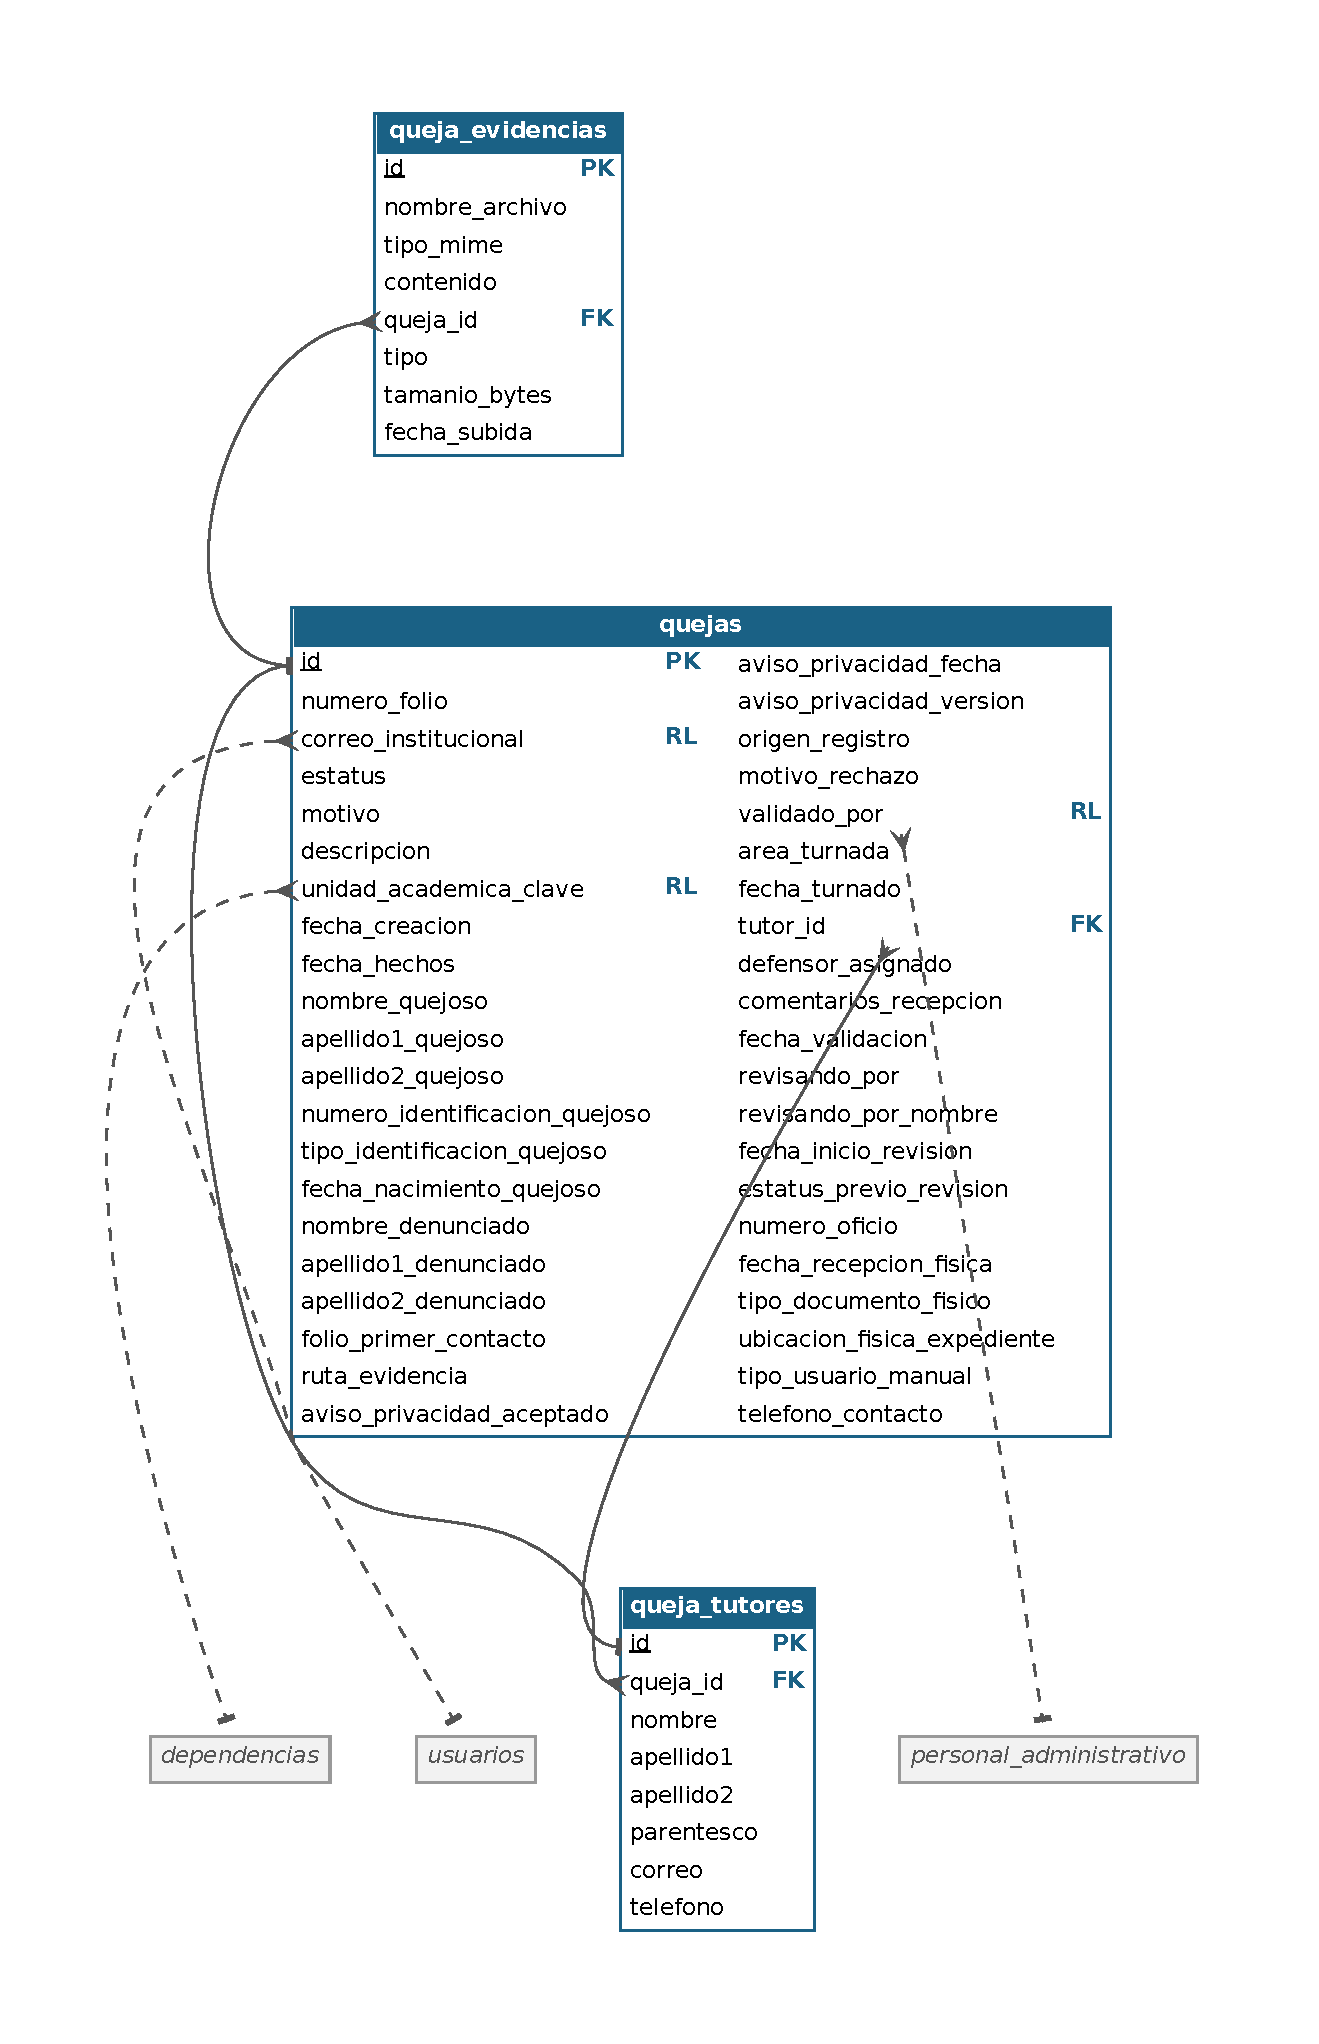
\includegraphics[width=\textwidth,height=0.85\textheight,keepaspectratio]{images/er_grupo_01.pdf}
	\caption{Diagrama entidad-relación: \texttt{quejas}, \texttt{queja\_tutores}, \texttt{queja\_evidencias}}
	\label{fig:er_grupo_01}
\end{figure}


\begin{figure}[H]
	\centering
	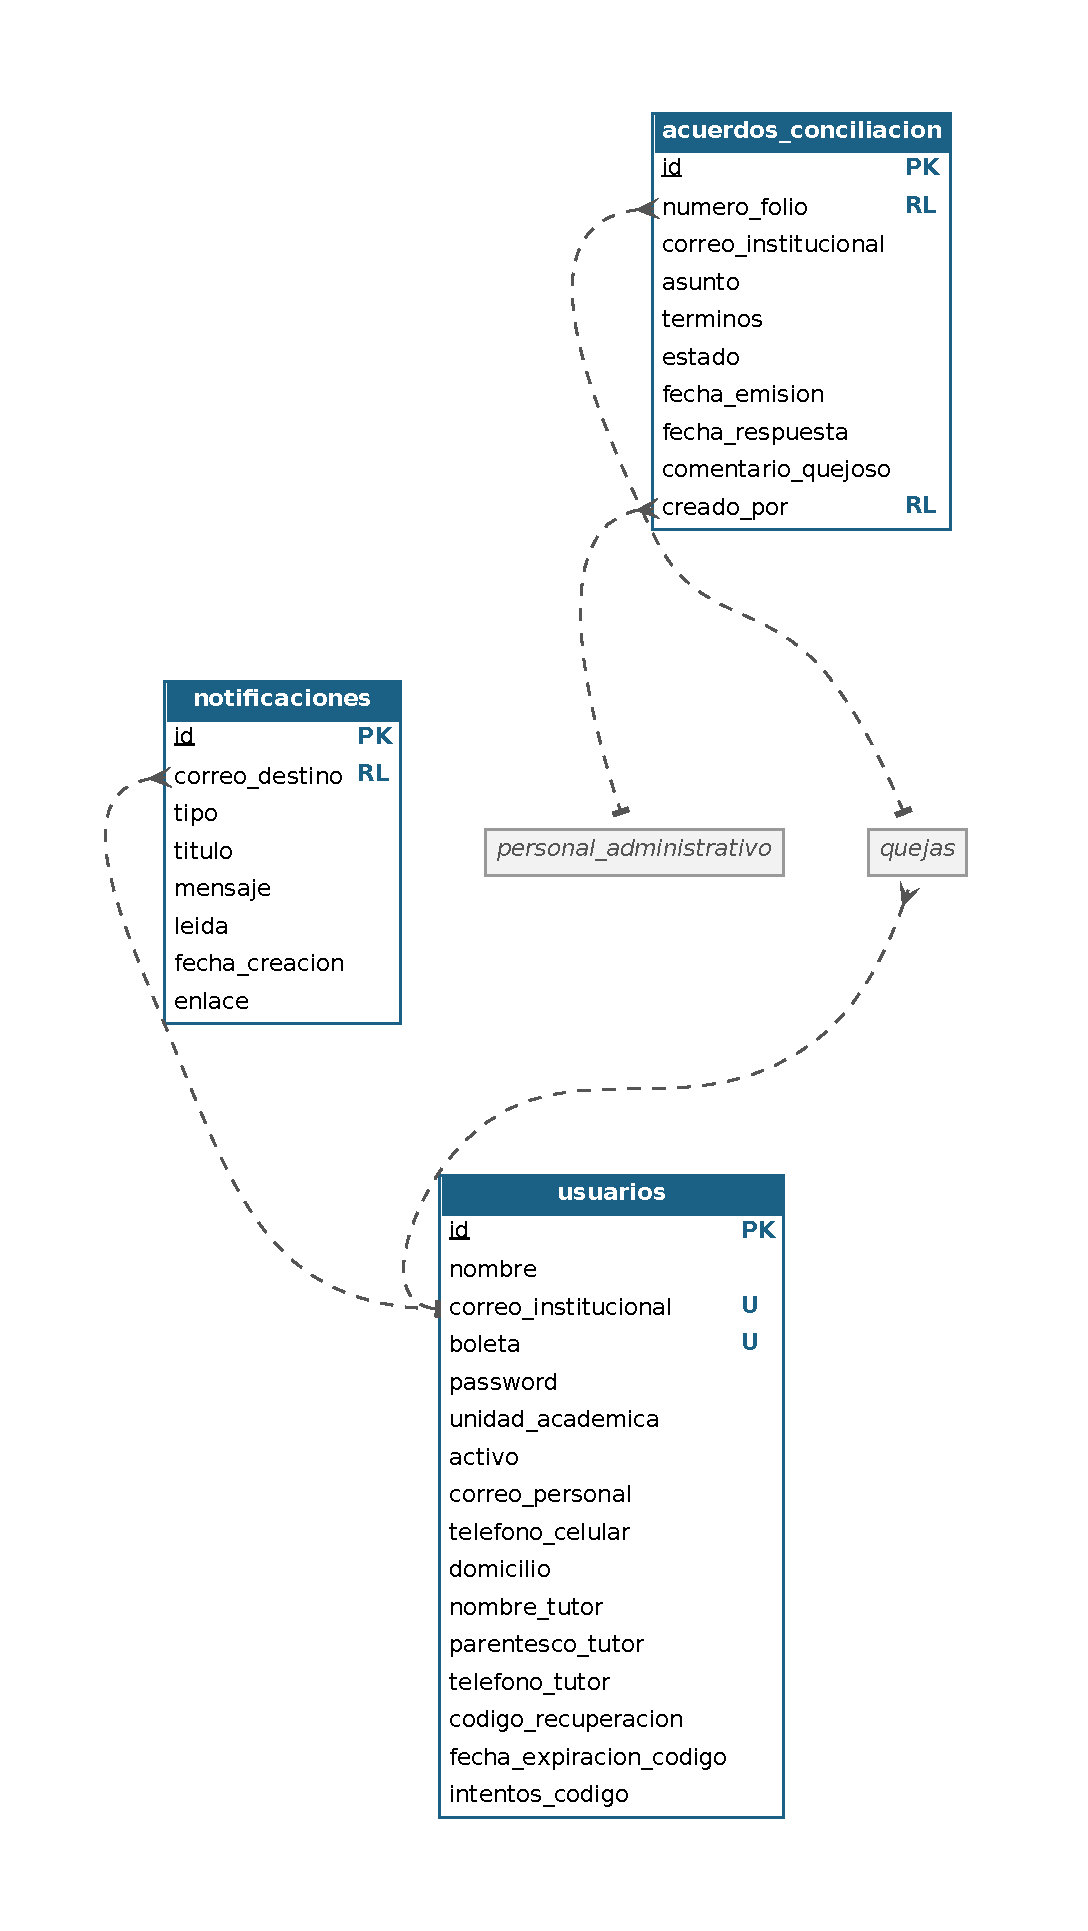
\includegraphics[width=\textwidth,height=0.85\textheight,keepaspectratio]{images/er_grupo_02.pdf}
	\caption{Diagrama entidad-relación: \texttt{usuarios}, \texttt{acuerdos\_conciliacion}, \texttt{notificaciones}}
	\label{fig:er_grupo_02}
\end{figure}

\subsection{Tabla \texttt{acuerdos\_conciliacion}}
Acuerdos de conciliación propuestos por la Defensoría y la respuesta del quejoso. Servicio responsable: revision-service, queja-service, primer-contacto-service.


\rowcolors{2}{rowblue}{white}
\footnotesize
\renewcommand{\arraystretch}{1.15}
\setlength{\tabcolsep}{4pt}
\begin{longtable}{|L{3.9cm}|L{2.4cm}|L{0.9cm}|L{1.2cm}|L{6.6cm}|}
	\hiderowcolors\caption{Diccionario de datos de la tabla \texttt{acuerdos\_conciliacion}}
	\label{tab:dic_acuerdos_conciliacion} \\ \showrowcolors
	\hline
	\rowcolor{headerblue}
	\headercell{Columna} & \headercell{Tipo} & \headercell{Nulo} & \headercell{Clave} & \headercell{Descripción} \\
	\hline
	\endfirsthead
	\hline
	\rowcolor{headerblue}
	\headercell{Columna} & \headercell{Tipo} & \headercell{Nulo} & \headercell{Clave} & \headercell{Descripción} \\
	\hline
	\endhead
		\texttt{id} & BIGINT & No & PK & Identificador único del registro, generado automáticamente. \\ \hline
		\texttt{numero\_\allowbreak{}folio} & VARCHAR(255) & No & RL & Folio de la queja a la que se dirige el acuerdo. \\ \hline
		\texttt{correo\_\allowbreak{}institucional} & VARCHAR(255) & No &  & Correo del quejoso destinatario; solo él puede responder. \\ \hline
		\texttt{asunto} & VARCHAR(255) & No &  & Asunto o tema del documento. \\ \hline
		\texttt{terminos} & TEXT & No &  & Términos del acuerdo. \\ \hline
		\texttt{estado} & VARCHAR(255) & No &  & Estado del acuerdo (pendiente, aceptado o rechazado). \\ \hline
		\texttt{fecha\_\allowbreak{}emision} & TIMESTAMP & Sí &  & Fecha y hora de emisión. \\ \hline
		\texttt{fecha\_\allowbreak{}respuesta} & TIMESTAMP & Sí &  & Fecha y hora de la respuesta. \\ \hline
		\texttt{comentario\_\allowbreak{}quejoso} & TEXT & Sí &  & Comentario del quejoso al responder. \\ \hline
		\texttt{creado\_\allowbreak{}por} & VARCHAR(255) & Sí & RL & Usuario que creó el registro. \\ \hline
\end{longtable}
\normalsize
\setlength{\tabcolsep}{6pt}
\renewcommand{\arraystretch}{1}

\subsection{Tabla \texttt{notificaciones}}
Avisos persistidos para cada destinatario, con su estado de lectura. Servicio responsable: notificaciones-service.


\rowcolors{2}{rowblue}{white}
\footnotesize
\renewcommand{\arraystretch}{1.15}
\setlength{\tabcolsep}{4pt}
\begin{longtable}{|L{3.9cm}|L{2.4cm}|L{0.9cm}|L{1.2cm}|L{6.6cm}|}
	\hiderowcolors\caption{Diccionario de datos de la tabla \texttt{notificaciones}}
	\label{tab:dic_notificaciones} \\ \showrowcolors
	\hline
	\rowcolor{headerblue}
	\headercell{Columna} & \headercell{Tipo} & \headercell{Nulo} & \headercell{Clave} & \headercell{Descripción} \\
	\hline
	\endfirsthead
	\hline
	\rowcolor{headerblue}
	\headercell{Columna} & \headercell{Tipo} & \headercell{Nulo} & \headercell{Clave} & \headercell{Descripción} \\
	\hline
	\endhead
		\texttt{id} & BIGINT & No & PK & Identificador único del registro, generado automáticamente. \\ \hline
		\texttt{correo\_\allowbreak{}destino} & VARCHAR(255) & No & RL & Correo electrónico del destinatario. \\ \hline
		\texttt{tipo} & VARCHAR(255) & No &  & Tipo de aviso. \\ \hline
		\texttt{titulo} & VARCHAR(255) & No &  & Título del aviso. \\ \hline
		\texttt{mensaje} & TEXT & Sí &  & Texto del aviso. \\ \hline
		\texttt{leida} & BOOLEAN & No &  & Indica si el aviso ya fue leído. \\ \hline
		\texttt{fecha\_\allowbreak{}creacion} & TIMESTAMP & Sí &  & Fecha y hora de creación del registro. \\ \hline
		\texttt{enlace} & VARCHAR(255) & Sí &  & Enlace de la plataforma relacionado con el aviso. \\ \hline
\end{longtable}
\normalsize
\setlength{\tabcolsep}{6pt}
\renewcommand{\arraystretch}{1}

\subsection{Tabla \texttt{queja\_evidencias}}
Archivos de evidencia adjuntos a una queja, almacenados con su contenido binario. Servicio responsable: queja-service.


\rowcolors{2}{rowblue}{white}
\footnotesize
\renewcommand{\arraystretch}{1.15}
\setlength{\tabcolsep}{4pt}
\begin{longtable}{|L{3.9cm}|L{2.4cm}|L{0.9cm}|L{1.2cm}|L{6.6cm}|}
	\hiderowcolors\caption{Diccionario de datos de la tabla \texttt{queja\_evidencias}}
	\label{tab:dic_queja_evidencias} \\ \showrowcolors
	\hline
	\rowcolor{headerblue}
	\headercell{Columna} & \headercell{Tipo} & \headercell{Nulo} & \headercell{Clave} & \headercell{Descripción} \\
	\hline
	\endfirsthead
	\hline
	\rowcolor{headerblue}
	\headercell{Columna} & \headercell{Tipo} & \headercell{Nulo} & \headercell{Clave} & \headercell{Descripción} \\
	\hline
	\endhead
		\texttt{id} & BIGINT & No & PK & Identificador único del registro, generado automáticamente. \\ \hline
		\texttt{nombre\_\allowbreak{}archivo} & VARCHAR(255) & No &  & Nombre original del archivo. \\ \hline
		\texttt{tipo\_\allowbreak{}mime} & VARCHAR(255) & Sí &  & Tipo MIME del archivo. \\ \hline
		\texttt{contenido} & BYTEA & No &  & Contenido binario del archivo. \\ \hline
		\texttt{queja\_\allowbreak{}id} & BIGINT & No & FK & Queja a la que pertenece el registro. \\ \hline
		\texttt{tipo} & VARCHAR(20) & Sí &  & Clasificación del archivo (evidencia o identificación). \\ \hline
		\texttt{tamanio\_\allowbreak{}bytes} & BIGINT & Sí &  & Tamaño del archivo en bytes. \\ \hline
		\texttt{fecha\_\allowbreak{}subida} & TIMESTAMP & Sí &  & Fecha y hora en que se subió el archivo. \\ \hline
\end{longtable}
\normalsize
\setlength{\tabcolsep}{6pt}
\renewcommand{\arraystretch}{1}

\subsection{Tabla \texttt{queja\_tutores}}
Datos del tutor o adulto responsable cuando el quejoso es menor de edad; relación uno a uno con la queja. Servicio responsable: queja-service.


\rowcolors{2}{rowblue}{white}
\footnotesize
\renewcommand{\arraystretch}{1.15}
\setlength{\tabcolsep}{4pt}
\begin{longtable}{|L{3.9cm}|L{2.4cm}|L{0.9cm}|L{1.2cm}|L{6.6cm}|}
	\hiderowcolors\caption{Diccionario de datos de la tabla \texttt{queja\_tutores}}
	\label{tab:dic_queja_tutores} \\ \showrowcolors
	\hline
	\rowcolor{headerblue}
	\headercell{Columna} & \headercell{Tipo} & \headercell{Nulo} & \headercell{Clave} & \headercell{Descripción} \\
	\hline
	\endfirsthead
	\hline
	\rowcolor{headerblue}
	\headercell{Columna} & \headercell{Tipo} & \headercell{Nulo} & \headercell{Clave} & \headercell{Descripción} \\
	\hline
	\endhead
		\texttt{id} & BIGINT & No & PK & Identificador único del registro, generado automáticamente. \\ \hline
		\texttt{queja\_\allowbreak{}id} & BIGINT & No & FK & Queja a la que pertenece el registro. \\ \hline
		\texttt{nombre} & VARCHAR(255) & Sí &  & Nombre del tutor. \\ \hline
		\texttt{apellido1} & VARCHAR(255) & Sí &  & Primer apellido. \\ \hline
		\texttt{apellido2} & VARCHAR(255) & Sí &  & Segundo apellido. \\ \hline
		\texttt{parentesco} & VARCHAR(255) & Sí &  & Parentesco con el quejoso. \\ \hline
		\texttt{correo} & VARCHAR(255) & Sí &  & Correo del tutor. \\ \hline
		\texttt{telefono} & VARCHAR(255) & Sí &  & Teléfono del tutor. \\ \hline
\end{longtable}
\normalsize
\setlength{\tabcolsep}{6pt}
\renewcommand{\arraystretch}{1}

\subsection{Tabla \texttt{quejas}}
Registro central de cada queja: folio, identidad del quejoso, narrativa de los hechos, persona señalada, estatus y datos del flujo de recepción (validación, rechazo y turnado). Es la tabla de la que parte todo el expediente. Servicio responsable: queja-service, revision-service, primer-contacto-service, subdefensoria-service.


\rowcolors{2}{rowblue}{white}
\footnotesize
\renewcommand{\arraystretch}{1.15}
\setlength{\tabcolsep}{4pt}
\begin{longtable}{|L{3.9cm}|L{2.4cm}|L{0.9cm}|L{1.2cm}|L{6.6cm}|}
	\hiderowcolors\caption{Diccionario de datos de la tabla \texttt{quejas}}
	\label{tab:dic_quejas} \\ \showrowcolors
	\hline
	\rowcolor{headerblue}
	\headercell{Columna} & \headercell{Tipo} & \headercell{Nulo} & \headercell{Clave} & \headercell{Descripción} \\
	\hline
	\endfirsthead
	\hline
	\rowcolor{headerblue}
	\headercell{Columna} & \headercell{Tipo} & \headercell{Nulo} & \headercell{Clave} & \headercell{Descripción} \\
	\hline
	\endhead
		\texttt{id} & BIGINT & No & PK & Identificador único del registro, generado automáticamente. \\ \hline
		\texttt{numero\_\allowbreak{}folio} & VARCHAR(255) & No &  & Folio de seguimiento que se entrega al quejoso. \\ \hline
		\texttt{correo\_\allowbreak{}institucional} & VARCHAR(255) & No & RL & Correo del quejoso; junto con el folio permite consultar la queja y activar la cuenta. \\ \hline
		\texttt{estatus} & VARCHAR(255) & Sí &  & Estatus de la queja (RECIBIDA, EN\_VALIDACION, RECHAZADA, TURNADA, entre otros). \\ \hline
		\texttt{motivo} & VARCHAR(255) & No &  & Motivo de la queja. \\ \hline
		\texttt{descripcion} & TEXT & Sí &  & Narrativa de los hechos redactada por el quejoso. \\ \hline
		\texttt{unidad\_\allowbreak{}academica\_\allowbreak{}clave} & VARCHAR(255) & Sí & RL & Clave de la unidad académica involucrada, tomada del catálogo. \\ \hline
		\texttt{fecha\_\allowbreak{}creacion} & TIMESTAMP & Sí &  & Fecha y hora en que se registró la queja. \\ \hline
		\texttt{fecha\_\allowbreak{}hechos} & DATE & Sí &  & Fecha en que ocurrieron los hechos. \\ \hline
		\texttt{nombre\_\allowbreak{}quejoso} & VARCHAR(255) & Sí &  & Nombre del quejoso. \\ \hline
		\texttt{apellido1\_\allowbreak{}quejoso} & VARCHAR(255) & Sí &  & Primer apellido del quejoso. \\ \hline
		\texttt{apellido2\_\allowbreak{}quejoso} & VARCHAR(255) & Sí &  & Segundo apellido del quejoso. \\ \hline
		\texttt{numero\_\allowbreak{}identificacion\_\allowbreak{}quejoso} & VARCHAR(255) & Sí &  & Número de boleta o de empleado del quejoso. \\ \hline
		\texttt{tipo\_\allowbreak{}identificacion\_\allowbreak{}quejoso} & VARCHAR(255) & Sí &  & Tipo de identificación del quejoso. \\ \hline
		\texttt{fecha\_\allowbreak{}nacimiento\_\allowbreak{}quejoso} & DATE & Sí &  & Fecha de nacimiento del quejoso, usada para identificar a menores de edad. \\ \hline
		\texttt{nombre\_\allowbreak{}denunciado} & VARCHAR(255) & Sí &  & Nombre de la persona señalada. \\ \hline
		\texttt{apellido1\_\allowbreak{}denunciado} & VARCHAR(255) & Sí &  & Primer apellido de la persona señalada. \\ \hline
		\texttt{apellido2\_\allowbreak{}denunciado} & VARCHAR(255) & Sí &  & Segundo apellido de la persona señalada. \\ \hline
		\texttt{folio\_\allowbreak{}primer\_\allowbreak{}contacto} & VARCHAR(255) & Sí &  & Folio asignado en Primer Contacto. \\ \hline
		\texttt{ruta\_\allowbreak{}evidencia} & VARCHAR(255) & Sí &  & Ruta de la evidencia principal de la queja. \\ \hline
		\texttt{aviso\_\allowbreak{}privacidad\_\allowbreak{}aceptado} & BOOLEAN & Sí &  & Indica si se aceptó el aviso de privacidad. \\ \hline
		\texttt{aviso\_\allowbreak{}privacidad\_\allowbreak{}fecha} & TIMESTAMP & Sí &  & Fecha y hora de aceptación del aviso de privacidad. \\ \hline
		\texttt{aviso\_\allowbreak{}privacidad\_\allowbreak{}version} & VARCHAR(255) & Sí &  & Versión del aviso de privacidad aceptada. \\ \hline
		\texttt{origen\_\allowbreak{}registro} & VARCHAR(255) & Sí &  & Punto de acceso por el que ingresó la queja (público, autenticado o manual). \\ \hline
		\texttt{motivo\_\allowbreak{}rechazo} & TEXT & Sí &  & Motivos y observaciones del rechazo. \\ \hline
		\texttt{validado\_\allowbreak{}por} & VARCHAR(255) & Sí & RL & Correo de la persona de Recepción que validó la queja. \\ \hline
		\texttt{area\_\allowbreak{}turnada} & VARCHAR(255) & Sí &  & Área a la que Recepción turnó la queja. \\ \hline
		\texttt{fecha\_\allowbreak{}turnado} & TIMESTAMP & Sí &  & Fecha y hora del turnado. \\ \hline
		\texttt{tutor\_\allowbreak{}id} & BIGINT & Sí & FK & Tutor asociado a la queja, cuando el quejoso es menor de edad. \\ \hline
		\texttt{defensor\_\allowbreak{}asignado} & VARCHAR(255) & Sí &  & Defensor o analista al que se asignó la queja al turnarla. \\ \hline
		\texttt{comentarios\_\allowbreak{}recepcion} & TEXT & Sí &  & Comentarios de Recepción al turnar la queja. \\ \hline
		\texttt{fecha\_\allowbreak{}validacion} & TIMESTAMP & Sí &  & Fecha y hora de la validación por Recepción. \\ \hline
		\texttt{revisando\_\allowbreak{}por} & VARCHAR(255) & Sí &  & Correo de la persona de Recepción que tiene tomada la queja. \\ \hline
		\texttt{revisando\_\allowbreak{}por\_\allowbreak{}nombre} & VARCHAR(255) & Sí &  & Nombre de la persona de Recepción que tiene tomada la queja. \\ \hline
		\texttt{fecha\_\allowbreak{}inicio\_\allowbreak{}revision} & TIMESTAMP & Sí &  & Fecha y hora en que Recepción tomó la queja para revisarla. \\ \hline
		\texttt{estatus\_\allowbreak{}previo\_\allowbreak{}revision} & VARCHAR(255) & Sí &  & Estatus que tenía la queja antes de que Recepción la tomara. \\ \hline
		\texttt{numero\_\allowbreak{}oficio} & VARCHAR(255) & Sí &  & Número del oficio. \\ \hline
		\texttt{fecha\_\allowbreak{}recepcion\_\allowbreak{}fisica} & DATE & Sí &  & Fecha de recepción del documento físico. \\ \hline
		\texttt{tipo\_\allowbreak{}documento\_\allowbreak{}fisico} & VARCHAR(255) & Sí &  & Tipo del documento físico recibido. \\ \hline
		\texttt{ubicacion\_\allowbreak{}fisica\_\allowbreak{}expediente} & VARCHAR(255) & Sí &  & Ubicación física del expediente en papel. \\ \hline
		\texttt{tipo\_\allowbreak{}usuario\_\allowbreak{}manual} & VARCHAR(255) & Sí &  & Tipo de usuario capturado en el registro manual. \\ \hline
		\texttt{telefono\_\allowbreak{}contacto} & VARCHAR(255) & Sí &  & Teléfono de contacto del quejoso. \\ \hline
\end{longtable}
\normalsize
\setlength{\tabcolsep}{6pt}
\renewcommand{\arraystretch}{1}

\subsection{Tabla \texttt{usuarios}}
Cuentas de seguimiento de los quejosos: identidad institucional, credencial cifrada, datos de contacto y código de recuperación. Servicio responsable: auth-service, queja-service.


\rowcolors{2}{rowblue}{white}
\footnotesize
\renewcommand{\arraystretch}{1.15}
\setlength{\tabcolsep}{4pt}
\begin{longtable}{|L{3.9cm}|L{2.4cm}|L{0.9cm}|L{1.2cm}|L{6.6cm}|}
	\hiderowcolors\caption{Diccionario de datos de la tabla \texttt{usuarios}}
	\label{tab:dic_usuarios} \\ \showrowcolors
	\hline
	\rowcolor{headerblue}
	\headercell{Columna} & \headercell{Tipo} & \headercell{Nulo} & \headercell{Clave} & \headercell{Descripción} \\
	\hline
	\endfirsthead
	\hline
	\rowcolor{headerblue}
	\headercell{Columna} & \headercell{Tipo} & \headercell{Nulo} & \headercell{Clave} & \headercell{Descripción} \\
	\hline
	\endhead
		\texttt{id} & BIGINT & No & PK & Identificador único del registro, generado automáticamente. \\ \hline
		\texttt{nombre} & VARCHAR(255) & No &  & Nombre completo del quejoso. \\ \hline
		\texttt{correo\_\allowbreak{}institucional} & VARCHAR(255) & No & U & Correo institucional del titular del registro. \\ \hline
		\texttt{boleta} & VARCHAR(255) & No & U & Número de boleta o de empleado del usuario. \\ \hline
		\texttt{password} & VARCHAR(255) & Sí &  & Contraseña cifrada mediante función de resumen. \\ \hline
		\texttt{unidad\_\allowbreak{}academica} & VARCHAR(255) & Sí &  & Unidad académica del quejoso. \\ \hline
		\texttt{activo} & BOOLEAN & Sí &  & Indica si la cuenta está activada. \\ \hline
		\texttt{correo\_\allowbreak{}personal} & VARCHAR(255) & Sí &  & Correo personal del quejoso. \\ \hline
		\texttt{telefono\_\allowbreak{}celular} & VARCHAR(255) & Sí &  & Teléfono celular del quejoso. \\ \hline
		\texttt{domicilio} & TEXT & Sí &  & Domicilio del quejoso. \\ \hline
		\texttt{nombre\_\allowbreak{}tutor} & VARCHAR(255) & Sí &  & Nombre del tutor del quejoso. \\ \hline
		\texttt{parentesco\_\allowbreak{}tutor} & VARCHAR(255) & Sí &  & Parentesco del tutor con el quejoso. \\ \hline
		\texttt{telefono\_\allowbreak{}tutor} & VARCHAR(255) & Sí &  & Teléfono del tutor. \\ \hline
		\texttt{codigo\_\allowbreak{}recuperacion} & VARCHAR(255) & Sí &  & Código de seis dígitos para restablecer la contraseña. \\ \hline
		\texttt{fecha\_\allowbreak{}expiracion\_\allowbreak{}codigo} & TIMESTAMP & Sí &  & Fecha y hora de expiración del código de recuperación. \\ \hline
		\texttt{intentos\_\allowbreak{}codigo} & INTEGER & Sí &  & Número de intentos fallidos con el código de recuperación. \\ \hline
\end{longtable}
\normalsize
\setlength{\tabcolsep}{6pt}
\renewcommand{\arraystretch}{1}

\section{Módulo: Primer Contacto}
\label{anx:bd_mod2}

Las figuras de esta sección muestran el diagrama entidad-relación del módulo con todas sus columnas, divididas en grupos de tablas para facilitar su lectura. Las tablas en gris pertenecen a otros grupos o módulos y se incluyen solo para mostrar las relaciones.


\begin{figure}[H]
	\centering
	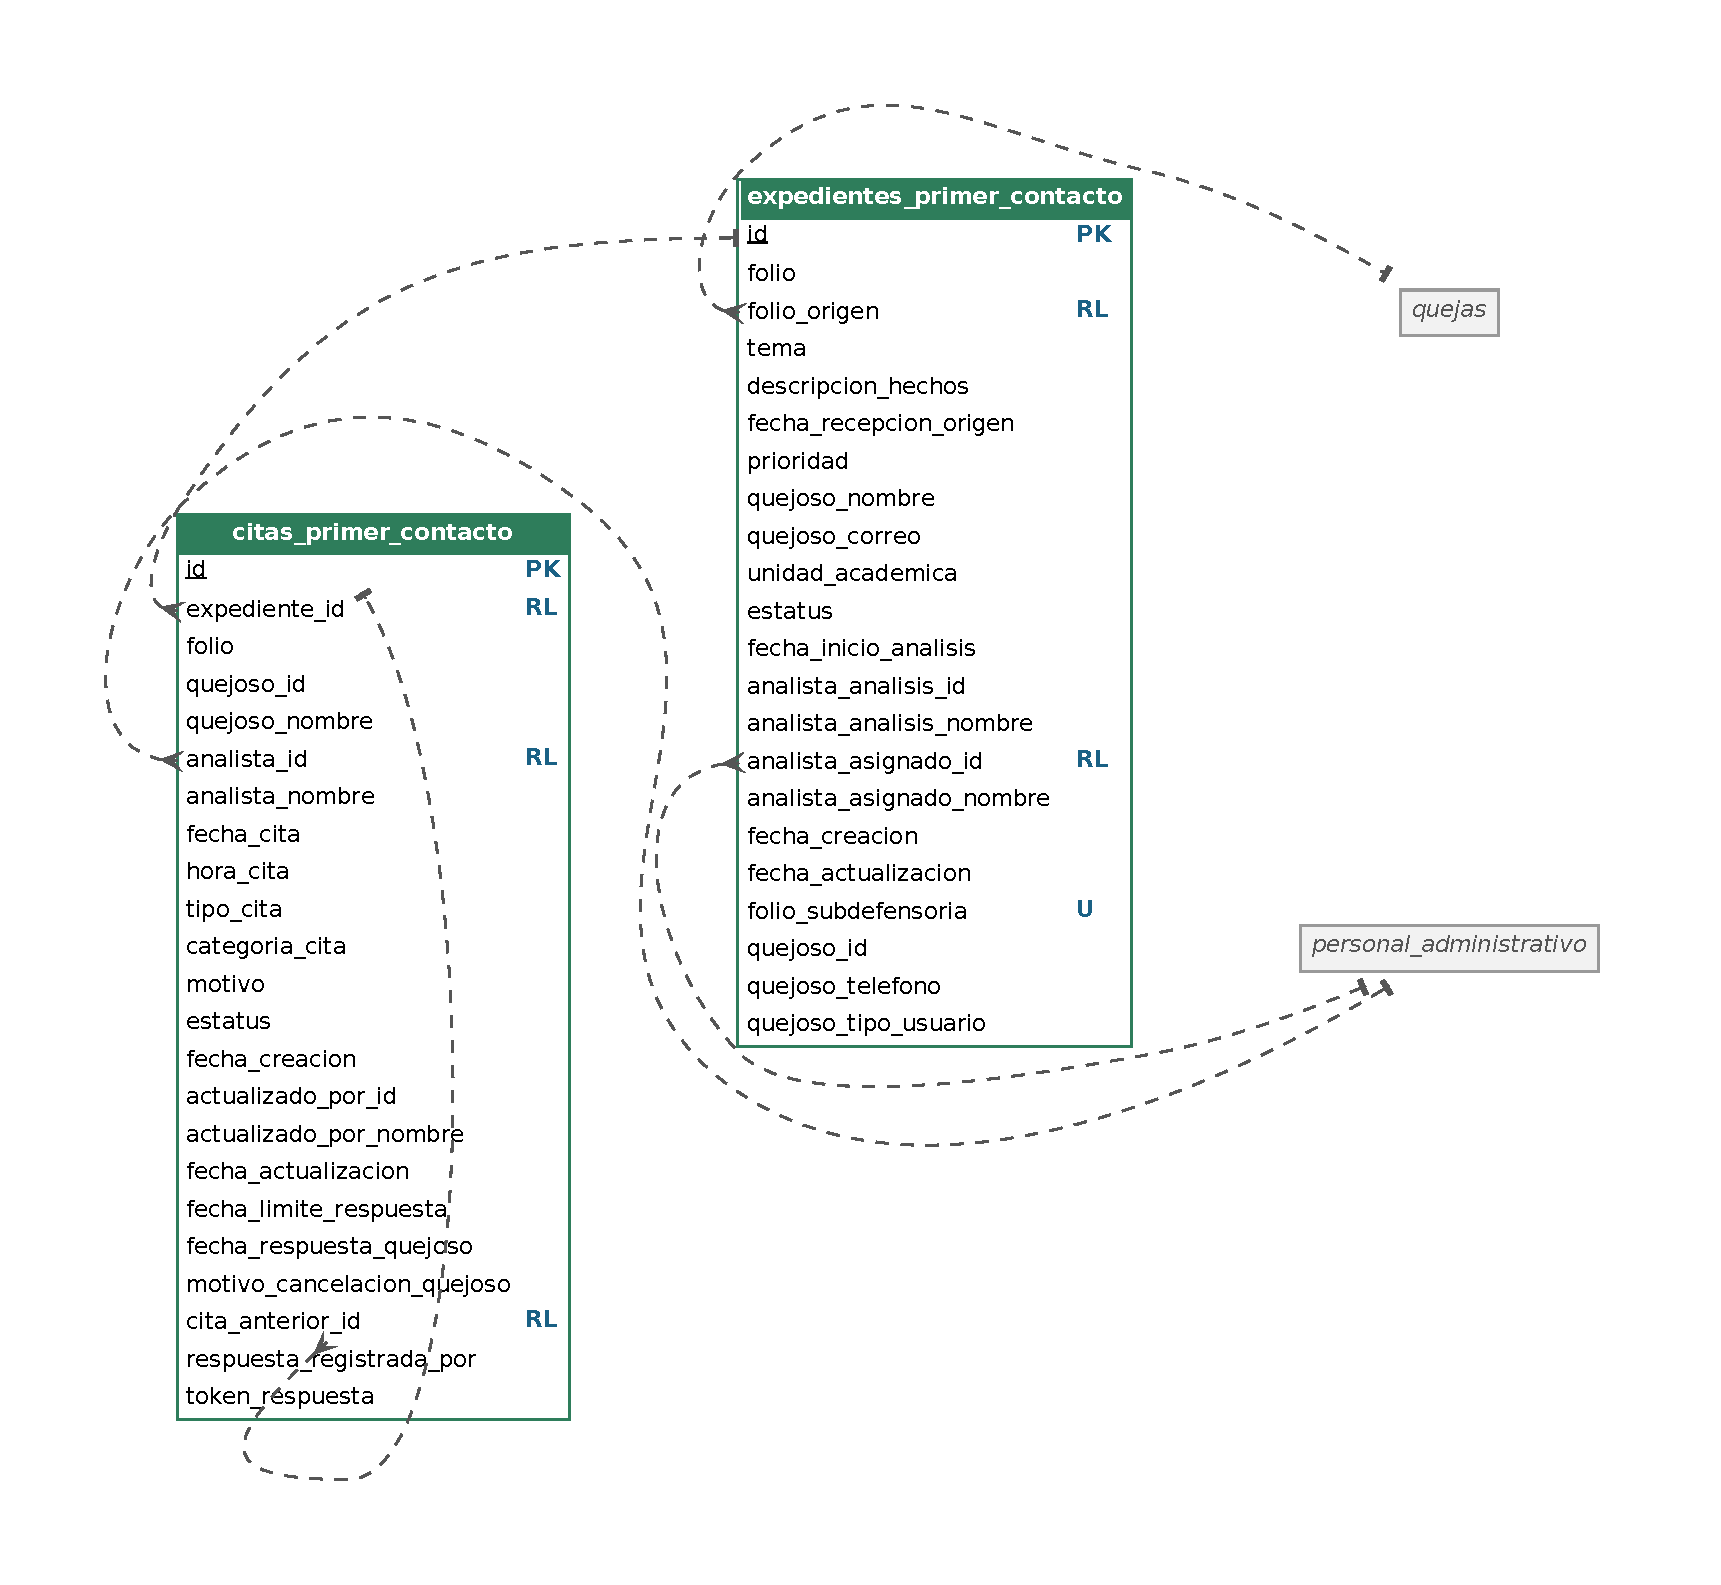
\includegraphics[width=\textwidth,height=0.85\textheight,keepaspectratio]{images/er_grupo_03.pdf}
	\caption{Diagrama entidad-relación: \texttt{expedientes\_primer\_contacto}, \texttt{citas\_primer\_contacto}}
	\label{fig:er_grupo_03}
\end{figure}


\begin{figure}[H]
	\centering
	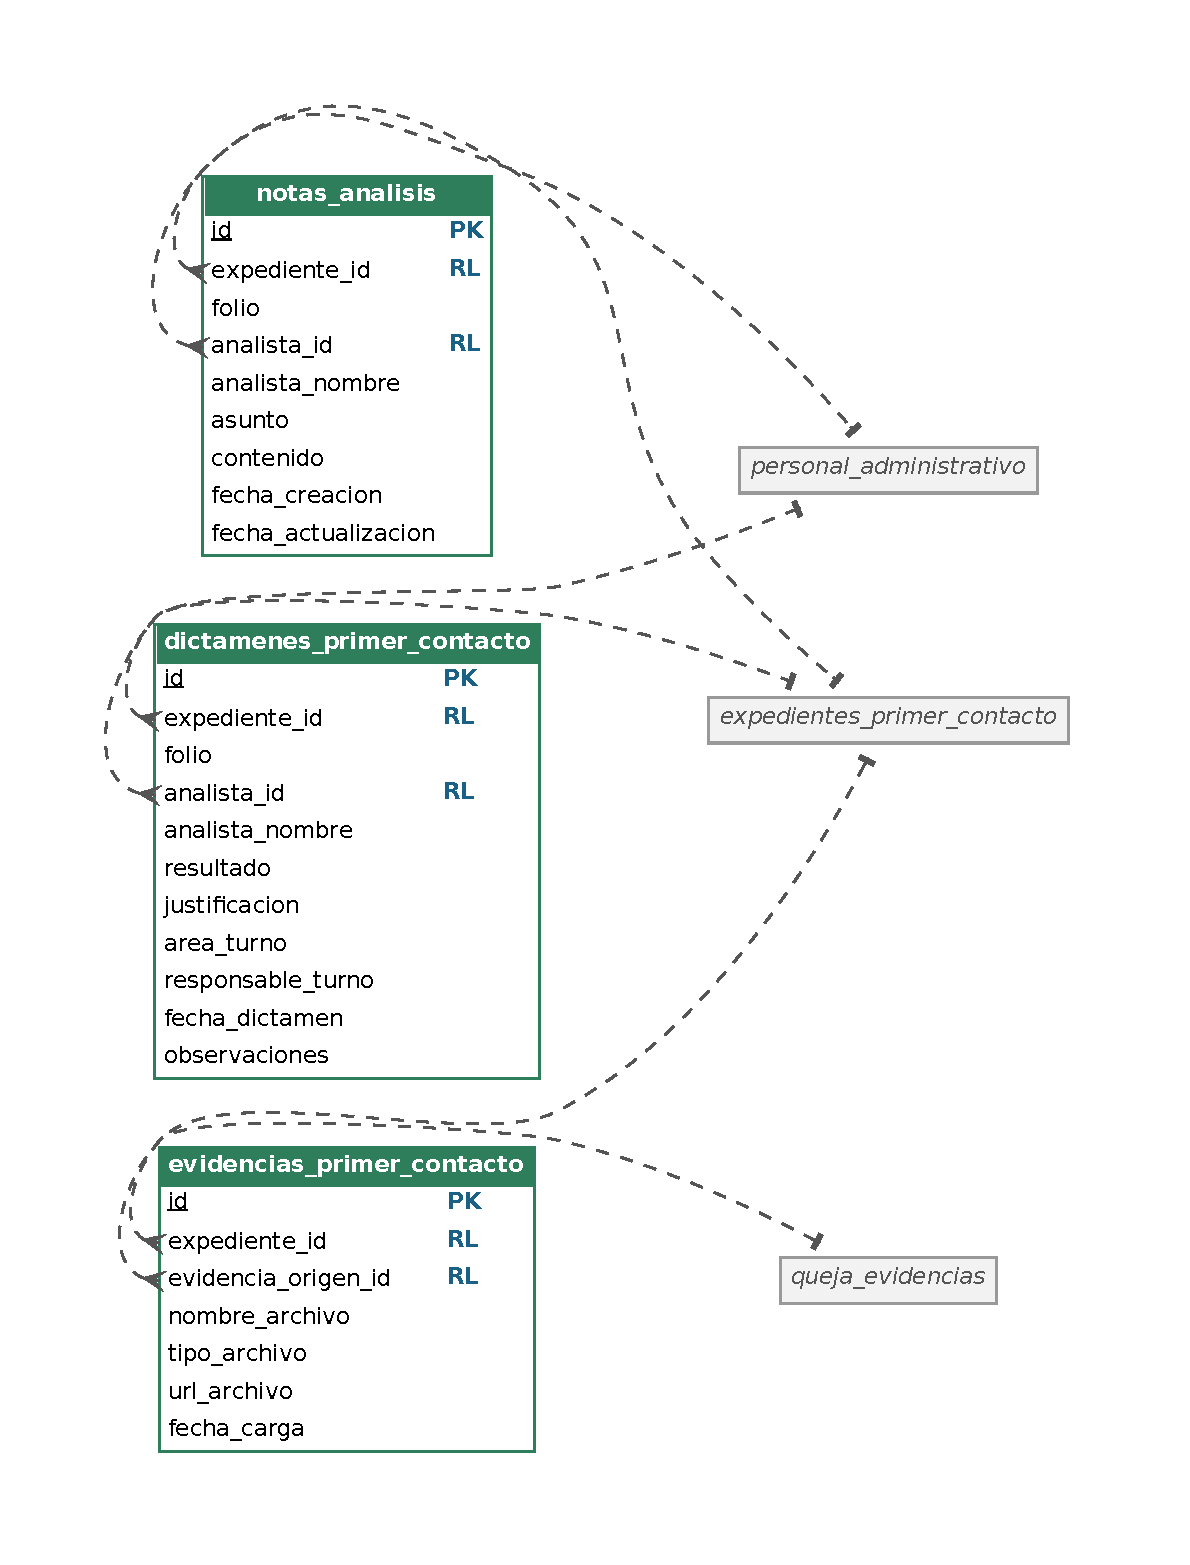
\includegraphics[width=\textwidth,height=0.85\textheight,keepaspectratio]{images/er_grupo_04.pdf}
	\caption{Diagrama entidad-relación: \texttt{dictamenes\_primer\_contacto}, \texttt{notas\_analisis}, \texttt{evidencias\_primer\_contacto}}
	\label{fig:er_grupo_04}
\end{figure}


\begin{figure}[H]
	\centering
	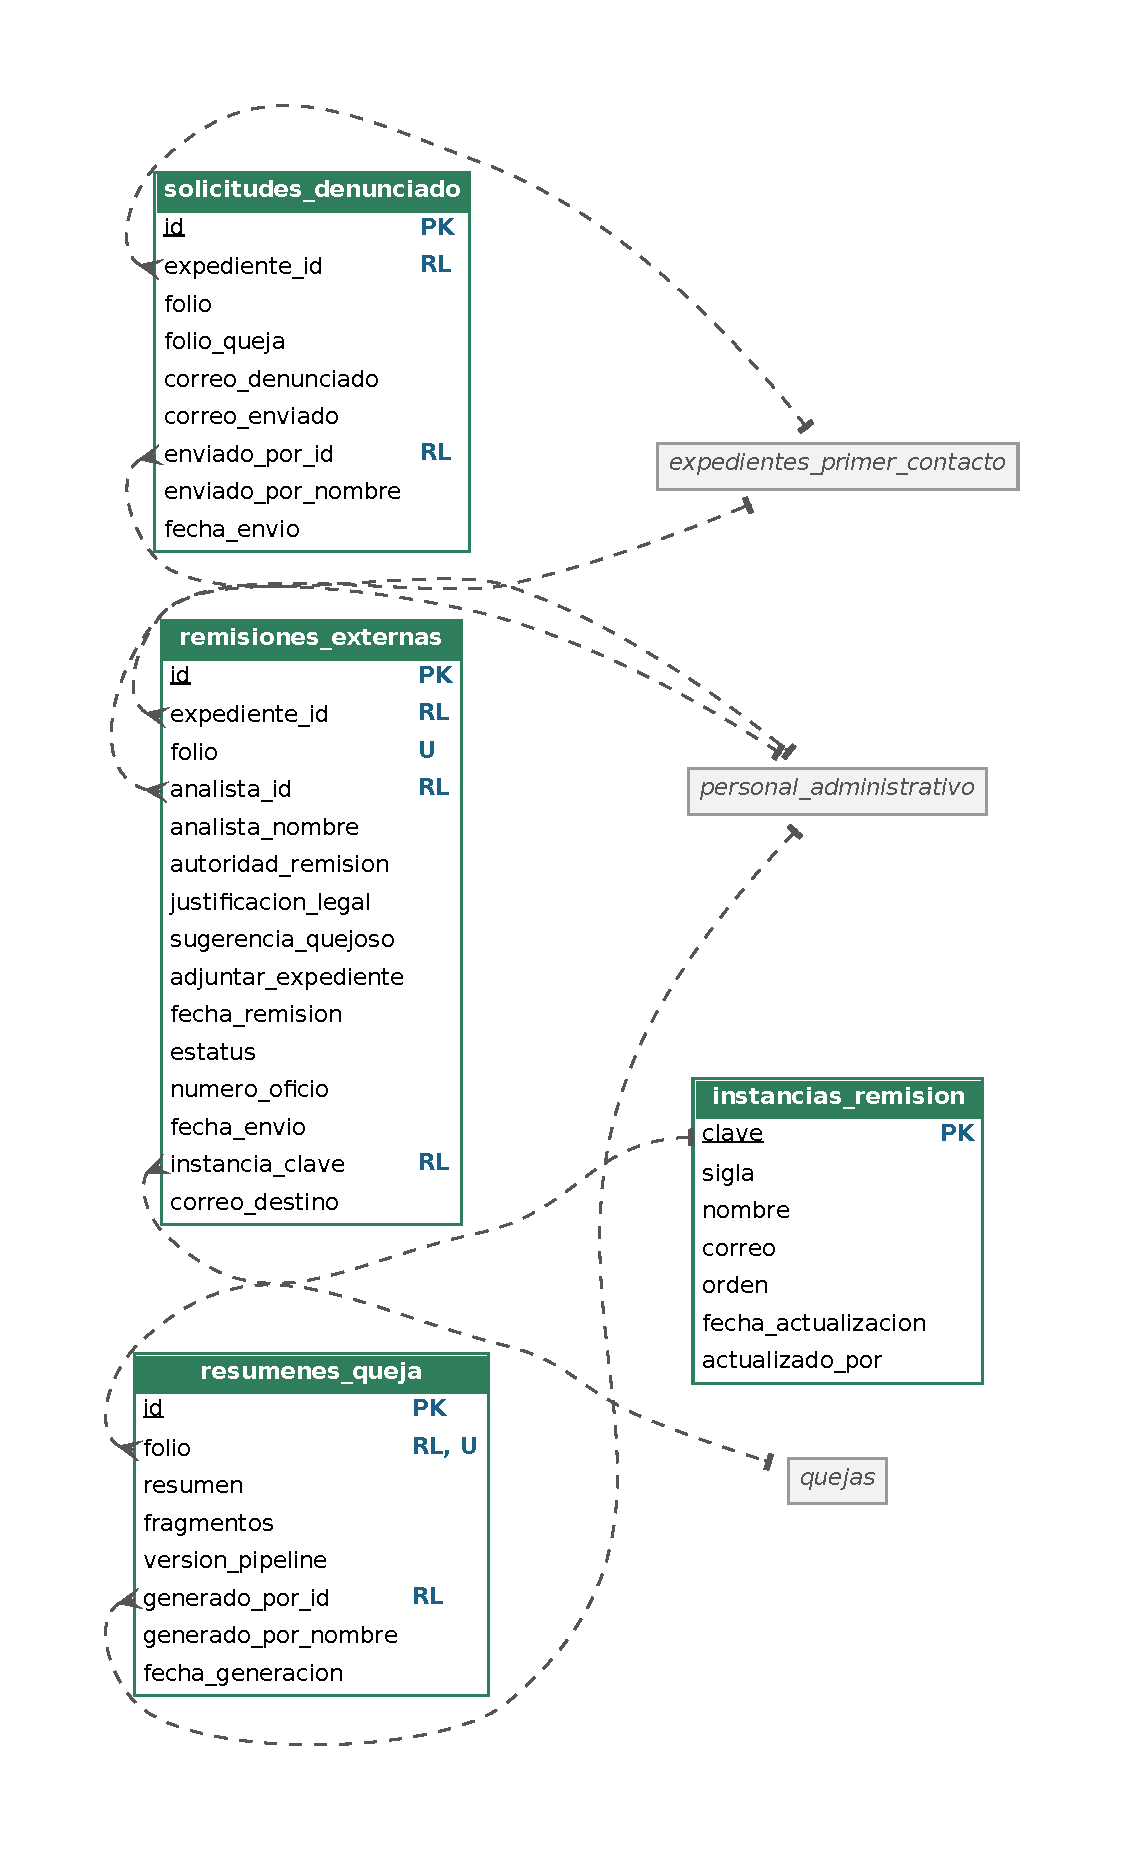
\includegraphics[width=\textwidth,height=0.85\textheight,keepaspectratio]{images/er_grupo_05.pdf}
	\caption{Diagrama entidad-relación: \texttt{remisiones\_externas}, \texttt{instancias\_remision}, \texttt{solicitudes\_denunciado}, \texttt{resumenes\_queja}}
	\label{fig:er_grupo_05}
\end{figure}


\begin{figure}[H]
	\centering
	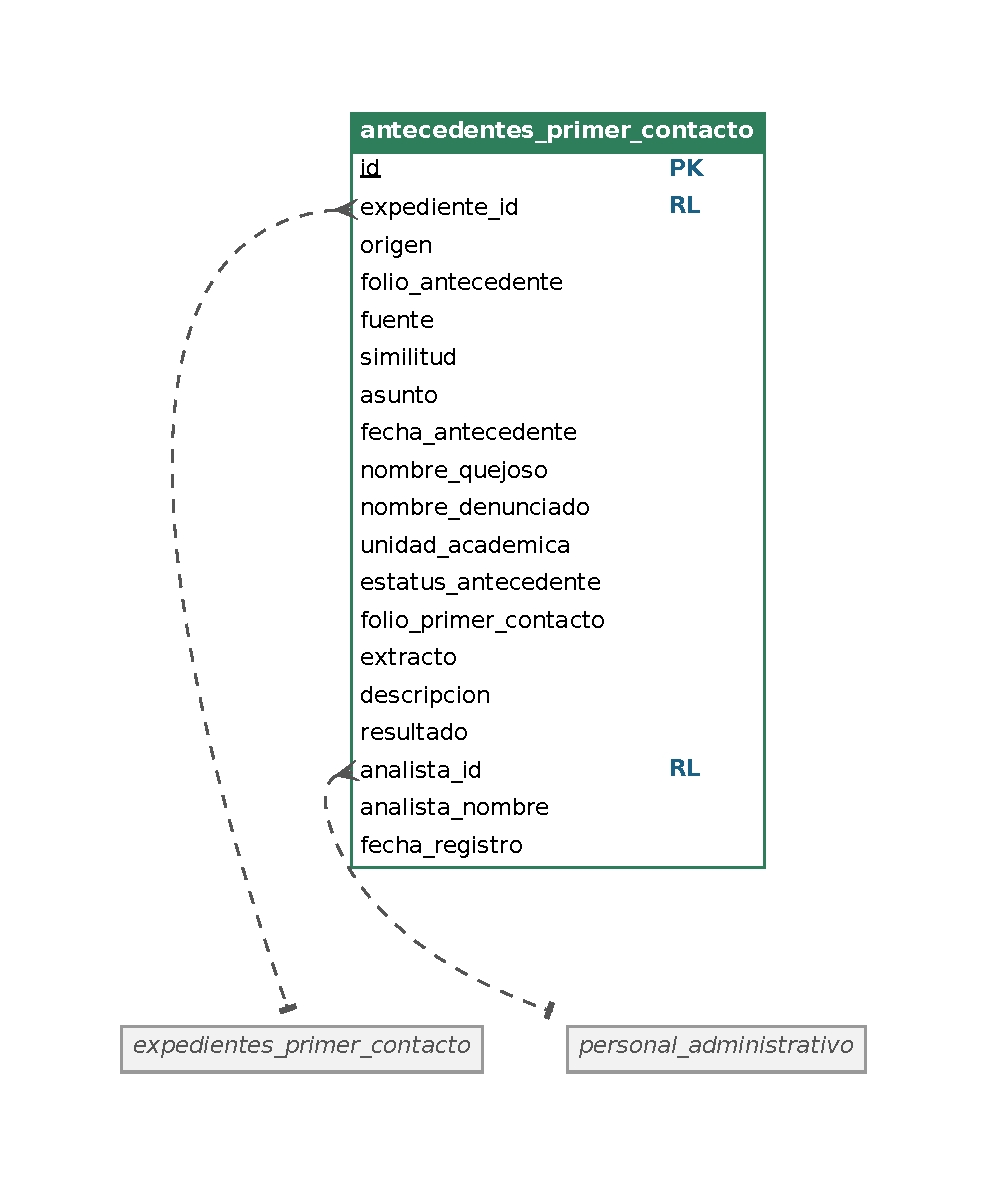
\includegraphics[width=\textwidth,height=0.85\textheight,keepaspectratio]{images/er_grupo_06.pdf}
	\caption{Diagrama entidad-relación: \texttt{antecedentes\_primer\_contacto}}
	\label{fig:er_grupo_06}
\end{figure}

\subsection{Tabla \texttt{antecedentes\_primer\_contacto}}
Antecedentes vinculados a un expediente, ya sea sugeridos por el modelo de búsqueda o agregados manualmente, con la decisión del analista. Servicio responsable: primer-contacto-service.


\rowcolors{2}{rowblue}{white}
\footnotesize
\renewcommand{\arraystretch}{1.15}
\setlength{\tabcolsep}{4pt}
\begin{longtable}{|L{3.9cm}|L{2.4cm}|L{0.9cm}|L{1.2cm}|L{6.6cm}|}
	\hiderowcolors\caption{Diccionario de datos de la tabla \texttt{antecedentes\_primer\_contacto}}
	\label{tab:dic_antecedentes_primer_contacto} \\ \showrowcolors
	\hline
	\rowcolor{headerblue}
	\headercell{Columna} & \headercell{Tipo} & \headercell{Nulo} & \headercell{Clave} & \headercell{Descripción} \\
	\hline
	\endfirsthead
	\hline
	\rowcolor{headerblue}
	\headercell{Columna} & \headercell{Tipo} & \headercell{Nulo} & \headercell{Clave} & \headercell{Descripción} \\
	\hline
	\endhead
		\texttt{id} & BIGINT & No & PK & Identificador único del registro, generado automáticamente. \\ \hline
		\texttt{expediente\_\allowbreak{}id} & BIGINT & No & RL & Expediente al que pertenece el registro. \\ \hline
		\texttt{origen} & VARCHAR(20) & No &  & Cómo se vinculó el antecedente (sugerido por el modelo o agregado manualmente). \\ \hline
		\texttt{folio\_\allowbreak{}antecedente} & VARCHAR(60) & No &  & Folio del expediente antecedente. \\ \hline
		\texttt{fuente} & VARCHAR(30) & No &  & Fuente del antecedente (base vigente o histórica). \\ \hline
		\texttt{similitud} & INTEGER & Sí &  & Porcentaje de similitud reportado por el modelo de antecedentes. \\ \hline
		\texttt{asunto} & VARCHAR(500) & Sí &  & Asunto o tema del documento. \\ \hline
		\texttt{fecha\_\allowbreak{}antecedente} & VARCHAR(30) & Sí &  & Fecha del expediente antecedente. \\ \hline
		\texttt{nombre\_\allowbreak{}quejoso} & VARCHAR(300) & Sí &  & Nombre del quejoso. \\ \hline
		\texttt{nombre\_\allowbreak{}denunciado} & VARCHAR(300) & Sí &  & Nombre de la persona señalada. \\ \hline
		\texttt{unidad\_\allowbreak{}academica} & VARCHAR(60) & Sí &  & Unidad académica relacionada. \\ \hline
		\texttt{estatus\_\allowbreak{}antecedente} & VARCHAR(50) & Sí &  & Estatus del expediente antecedente al momento de vincularlo. \\ \hline
		\texttt{folio\_\allowbreak{}primer\_\allowbreak{}contacto} & VARCHAR(50) & Sí &  & Folio asignado en Primer Contacto. \\ \hline
		\texttt{extracto} & TEXT & Sí &  & Fragmento del antecedente que coincide con la queja. \\ \hline
		\texttt{descripcion} & TEXT & Sí &  & Narrativa del expediente antecedente. \\ \hline
		\texttt{resultado} & VARCHAR(50) & Sí &  & Decisión del analista sobre el antecedente. \\ \hline
		\texttt{analista\_\allowbreak{}id} & BIGINT & No & RL & Identificador del analista que registró el elemento. \\ \hline
		\texttt{analista\_\allowbreak{}nombre} & VARCHAR(150) & Sí &  & Nombre del analista que registró el elemento. \\ \hline
		\texttt{fecha\_\allowbreak{}registro} & TIMESTAMP & No &  & Fecha y hora del registro. \\ \hline
\end{longtable}
\normalsize
\setlength{\tabcolsep}{6pt}
\renewcommand{\arraystretch}{1}

\subsection{Tabla \texttt{citas\_primer\_contacto}}
Citas programadas con el quejoso o con la persona señalada durante el análisis, con su estado y la respuesta de la persona citada. Servicio responsable: primer-contacto-service.


\rowcolors{2}{rowblue}{white}
\footnotesize
\renewcommand{\arraystretch}{1.15}
\setlength{\tabcolsep}{4pt}
\begin{longtable}{|L{3.9cm}|L{2.4cm}|L{0.9cm}|L{1.2cm}|L{6.6cm}|}
	\hiderowcolors\caption{Diccionario de datos de la tabla \texttt{citas\_primer\_contacto}}
	\label{tab:dic_citas_primer_contacto} \\ \showrowcolors
	\hline
	\rowcolor{headerblue}
	\headercell{Columna} & \headercell{Tipo} & \headercell{Nulo} & \headercell{Clave} & \headercell{Descripción} \\
	\hline
	\endfirsthead
	\hline
	\rowcolor{headerblue}
	\headercell{Columna} & \headercell{Tipo} & \headercell{Nulo} & \headercell{Clave} & \headercell{Descripción} \\
	\hline
	\endhead
		\texttt{id} & BIGINT & No & PK & Identificador único del registro, generado automáticamente. \\ \hline
		\texttt{expediente\_\allowbreak{}id} & BIGINT & No & RL & Expediente al que pertenece el registro. \\ \hline
		\texttt{folio} & VARCHAR(50) & No &  & Folio del expediente de Primer Contacto. \\ \hline
		\texttt{quejoso\_\allowbreak{}id} & BIGINT & Sí &  & Identificador de la cuenta del quejoso, si existe. \\ \hline
		\texttt{quejoso\_\allowbreak{}nombre} & VARCHAR(150) & Sí &  & Nombre del quejoso. \\ \hline
		\texttt{analista\_\allowbreak{}id} & BIGINT & No & RL & Identificador del analista que registró el elemento. \\ \hline
		\texttt{analista\_\allowbreak{}nombre} & VARCHAR(150) & Sí &  & Nombre del analista que registró el elemento. \\ \hline
		\texttt{fecha\_\allowbreak{}cita} & DATE & No &  & Fecha de la cita. \\ \hline
		\texttt{hora\_\allowbreak{}cita} & TIME & No &  & Hora de la cita. \\ \hline
		\texttt{tipo\_\allowbreak{}cita} & VARCHAR(50) & No &  & Tipo de cita (comparecencia, revisión de documentos o seguimiento). \\ \hline
		\texttt{categoria\_\allowbreak{}cita} & VARCHAR(30) & Sí &  & Persona con la que se agenda la cita (quejoso o persona señalada). \\ \hline
		\texttt{motivo} & TEXT & No &  & Motivo de la cita. \\ \hline
		\texttt{estatus} & VARCHAR(50) & No &  & Estado de la cita (programada, confirmada, reagendada, cancelada, etc.). \\ \hline
		\texttt{fecha\_\allowbreak{}creacion} & TIMESTAMP & No &  & Fecha y hora de creación del registro. \\ \hline
		\texttt{actualizado\_\allowbreak{}por\_\allowbreak{}id} & BIGINT & Sí &  & Identificador del usuario que realizó la última actualización. \\ \hline
		\texttt{actualizado\_\allowbreak{}por\_\allowbreak{}nombre} & VARCHAR(150) & Sí &  & Nombre del usuario que realizó la última actualización. \\ \hline
		\texttt{fecha\_\allowbreak{}actualizacion} & TIMESTAMP & Sí &  & Fecha y hora de la última actualización. \\ \hline
		\texttt{fecha\_\allowbreak{}limite\_\allowbreak{}respuesta} & TIMESTAMP & Sí &  & Fecha límite para que la persona citada responda. \\ \hline
		\texttt{fecha\_\allowbreak{}respuesta\_\allowbreak{}quejoso} & TIMESTAMP & Sí &  & Fecha y hora de la respuesta del quejoso. \\ \hline
		\texttt{motivo\_\allowbreak{}cancelacion\_\allowbreak{}quejoso} & TEXT & Sí &  & Motivo por el que la persona citada canceló. \\ \hline
		\texttt{cita\_\allowbreak{}anterior\_\allowbreak{}id} & BIGINT & Sí & RL & Cita original cuando la actual es una reprogramación. \\ \hline
		\texttt{respuesta\_\allowbreak{}registrada\_\allowbreak{}por} & VARCHAR(20) & Sí &  & Quién registró la respuesta (la persona citada o el analista). \\ \hline
		\texttt{token\_\allowbreak{}respuesta} & VARCHAR(64) & Sí &  & Token del enlace con el que la persona responde sin iniciar sesión. \\ \hline
\end{longtable}
\normalsize
\setlength{\tabcolsep}{6pt}
\renewcommand{\arraystretch}{1}

\subsection{Tabla \texttt{dictamenes\_primer\_contacto}}
Dictamen de competencia del expediente (procedente o improcedente) con su justificación. Servicio responsable: primer-contacto-service.


\rowcolors{2}{rowblue}{white}
\footnotesize
\renewcommand{\arraystretch}{1.15}
\setlength{\tabcolsep}{4pt}
\begin{longtable}{|L{3.9cm}|L{2.4cm}|L{0.9cm}|L{1.2cm}|L{6.6cm}|}
	\hiderowcolors\caption{Diccionario de datos de la tabla \texttt{dictamenes\_primer\_contacto}}
	\label{tab:dic_dictamenes_primer_contacto} \\ \showrowcolors
	\hline
	\rowcolor{headerblue}
	\headercell{Columna} & \headercell{Tipo} & \headercell{Nulo} & \headercell{Clave} & \headercell{Descripción} \\
	\hline
	\endfirsthead
	\hline
	\rowcolor{headerblue}
	\headercell{Columna} & \headercell{Tipo} & \headercell{Nulo} & \headercell{Clave} & \headercell{Descripción} \\
	\hline
	\endhead
		\texttt{id} & BIGINT & No & PK & Identificador único del registro, generado automáticamente. \\ \hline
		\texttt{expediente\_\allowbreak{}id} & BIGINT & No & RL & Expediente al que pertenece el registro. \\ \hline
		\texttt{folio} & VARCHAR(50) & No &  & Folio del expediente de Primer Contacto. \\ \hline
		\texttt{analista\_\allowbreak{}id} & BIGINT & No & RL & Identificador del analista que registró el elemento. \\ \hline
		\texttt{analista\_\allowbreak{}nombre} & VARCHAR(150) & Sí &  & Nombre del analista que registró el elemento. \\ \hline
		\texttt{resultado} & VARCHAR(50) & No &  & Sentido del dictamen (procedente o improcedente). \\ \hline
		\texttt{justificacion} & TEXT & No &  & Justificación del dictamen. \\ \hline
		\texttt{area\_\allowbreak{}turno} & VARCHAR(150) & Sí &  & Área a la que se turna el expediente dictaminado. \\ \hline
		\texttt{responsable\_\allowbreak{}turno} & VARCHAR(150) & Sí &  & Responsable al que se turna el expediente. \\ \hline
		\texttt{fecha\_\allowbreak{}dictamen} & TIMESTAMP & No &  & Fecha y hora del dictamen. \\ \hline
		\texttt{observaciones} & TEXT & Sí &  & Observaciones adicionales. \\ \hline
\end{longtable}
\normalsize
\setlength{\tabcolsep}{6pt}
\renewcommand{\arraystretch}{1}

\subsection{Tabla \texttt{evidencias\_primer\_contacto}}
Referencias a las evidencias disponibles en el expediente de análisis. Servicio responsable: primer-contacto-service.


\rowcolors{2}{rowblue}{white}
\footnotesize
\renewcommand{\arraystretch}{1.15}
\setlength{\tabcolsep}{4pt}
\begin{longtable}{|L{3.9cm}|L{2.4cm}|L{0.9cm}|L{1.2cm}|L{6.6cm}|}
	\hiderowcolors\caption{Diccionario de datos de la tabla \texttt{evidencias\_primer\_contacto}}
	\label{tab:dic_evidencias_primer_contacto} \\ \showrowcolors
	\hline
	\rowcolor{headerblue}
	\headercell{Columna} & \headercell{Tipo} & \headercell{Nulo} & \headercell{Clave} & \headercell{Descripción} \\
	\hline
	\endfirsthead
	\hline
	\rowcolor{headerblue}
	\headercell{Columna} & \headercell{Tipo} & \headercell{Nulo} & \headercell{Clave} & \headercell{Descripción} \\
	\hline
	\endhead
		\texttt{id} & BIGINT & No & PK & Identificador único del registro, generado automáticamente. \\ \hline
		\texttt{expediente\_\allowbreak{}id} & BIGINT & No & RL & Expediente al que pertenece el registro. \\ \hline
		\texttt{evidencia\_\allowbreak{}origen\_\allowbreak{}id} & BIGINT & Sí & RL & Evidencia de la queja de la que proviene el registro. \\ \hline
		\texttt{nombre\_\allowbreak{}archivo} & VARCHAR(255) & Sí &  & Nombre original del archivo. \\ \hline
		\texttt{tipo\_\allowbreak{}archivo} & VARCHAR(100) & Sí &  & Tipo del archivo. \\ \hline
		\texttt{url\_\allowbreak{}archivo} & VARCHAR(1000) & Sí &  & Ubicación del archivo. \\ \hline
		\texttt{fecha\_\allowbreak{}carga} & VARCHAR(50) & Sí &  & Fecha de carga del archivo. \\ \hline
\end{longtable}
\normalsize
\setlength{\tabcolsep}{6pt}
\renewcommand{\arraystretch}{1}

\subsection{Tabla \texttt{expedientes\_primer\_contacto}}
Expediente de análisis que se crea cuando Recepción turna una queja; concentra el estado del análisis, el analista asignado y el vínculo con Subdefensoría. Servicio responsable: primer-contacto-service.


\rowcolors{2}{rowblue}{white}
\footnotesize
\renewcommand{\arraystretch}{1.15}
\setlength{\tabcolsep}{4pt}
\begin{longtable}{|L{3.9cm}|L{2.4cm}|L{0.9cm}|L{1.2cm}|L{6.6cm}|}
	\hiderowcolors\caption{Diccionario de datos de la tabla \texttt{expedientes\_primer\_contacto}}
	\label{tab:dic_expedientes_primer_contacto} \\ \showrowcolors
	\hline
	\rowcolor{headerblue}
	\headercell{Columna} & \headercell{Tipo} & \headercell{Nulo} & \headercell{Clave} & \headercell{Descripción} \\
	\hline
	\endfirsthead
	\hline
	\rowcolor{headerblue}
	\headercell{Columna} & \headercell{Tipo} & \headercell{Nulo} & \headercell{Clave} & \headercell{Descripción} \\
	\hline
	\endhead
		\texttt{id} & BIGINT & No & PK & Identificador único del registro, generado automáticamente. \\ \hline
		\texttt{folio} & VARCHAR(50) & No &  & Folio del expediente en Primer Contacto. \\ \hline
		\texttt{folio\_\allowbreak{}origen} & VARCHAR(50) & No & RL & Folio de la queja original. \\ \hline
		\texttt{tema} & VARCHAR(200) & Sí &  & Tema o motivo de la queja. \\ \hline
		\texttt{descripcion\_\allowbreak{}hechos} & TEXT & Sí &  & Narrativa de los hechos copiada de la queja. \\ \hline
		\texttt{fecha\_\allowbreak{}recepcion\_\allowbreak{}origen} & VARCHAR(50) & Sí &  & Fecha de recepción de la queja original. \\ \hline
		\texttt{prioridad} & VARCHAR(30) & Sí &  & Prioridad del expediente (baja, media, alta o urgente). \\ \hline
		\texttt{quejoso\_\allowbreak{}nombre} & VARCHAR(200) & Sí &  & Nombre del quejoso. \\ \hline
		\texttt{quejoso\_\allowbreak{}correo} & VARCHAR(150) & Sí &  & Correo electrónico del quejoso. \\ \hline
		\texttt{unidad\_\allowbreak{}academica} & VARCHAR(200) & Sí &  & Unidad académica relacionada. \\ \hline
		\texttt{estatus} & VARCHAR(40) & No &  & Estatus del análisis (TURNADA, EN\_ANALISIS, PROCEDENTE, IMPROCEDENTE, REMITIDA, entre otros). \\ \hline
		\texttt{fecha\_\allowbreak{}inicio\_\allowbreak{}analisis} & TIMESTAMP & Sí &  & Fecha y hora en que inició el análisis. \\ \hline
		\texttt{analista\_\allowbreak{}analisis\_\allowbreak{}id} & BIGINT & Sí &  & Identificador del analista que inició el análisis. \\ \hline
		\texttt{analista\_\allowbreak{}analisis\_\allowbreak{}nombre} & VARCHAR(150) & Sí &  & Nombre del analista que inició el análisis. \\ \hline
		\texttt{analista\_\allowbreak{}asignado\_\allowbreak{}id} & BIGINT & Sí & RL & Identificador del analista al que Recepción turnó el expediente. \\ \hline
		\texttt{analista\_\allowbreak{}asignado\_\allowbreak{}nombre} & VARCHAR(150) & Sí &  & Nombre del analista asignado. \\ \hline
		\texttt{fecha\_\allowbreak{}creacion} & TIMESTAMP & No &  & Fecha y hora de creación del registro. \\ \hline
		\texttt{fecha\_\allowbreak{}actualizacion} & TIMESTAMP & Sí &  & Fecha y hora de la última actualización. \\ \hline
		\texttt{folio\_\allowbreak{}subdefensoria} & VARCHAR(50) & Sí & U & Folio del expediente de investigación en Subdefensoría. \\ \hline
		\texttt{quejoso\_\allowbreak{}id} & BIGINT & Sí &  & Identificador de la cuenta del quejoso, si existe. \\ \hline
		\texttt{quejoso\_\allowbreak{}telefono} & VARCHAR(30) & Sí &  & Teléfono del quejoso. \\ \hline
		\texttt{quejoso\_\allowbreak{}tipo\_\allowbreak{}usuario} & VARCHAR(50) & Sí &  & Tipo de usuario del quejoso (alumno, personal, etc.). \\ \hline
\end{longtable}
\normalsize
\setlength{\tabcolsep}{6pt}
\renewcommand{\arraystretch}{1}

\subsection{Tabla \texttt{instancias\_remision}}
Catálogo de instancias a las que se puede remitir un asunto improcedente (Abogado General, Órgano Interno de Control, entre otras). Servicio responsable: catalogo-service, primer-contacto-service.


\rowcolors{2}{rowblue}{white}
\footnotesize
\renewcommand{\arraystretch}{1.15}
\setlength{\tabcolsep}{4pt}
\begin{longtable}{|L{3.9cm}|L{2.4cm}|L{0.9cm}|L{1.2cm}|L{6.6cm}|}
	\hiderowcolors\caption{Diccionario de datos de la tabla \texttt{instancias\_remision}}
	\label{tab:dic_instancias_remision} \\ \showrowcolors
	\hline
	\rowcolor{headerblue}
	\headercell{Columna} & \headercell{Tipo} & \headercell{Nulo} & \headercell{Clave} & \headercell{Descripción} \\
	\hline
	\endfirsthead
	\hline
	\rowcolor{headerblue}
	\headercell{Columna} & \headercell{Tipo} & \headercell{Nulo} & \headercell{Clave} & \headercell{Descripción} \\
	\hline
	\endhead
		\texttt{clave} & VARCHAR(30) & No & PK & Clave única de la instancia. \\ \hline
		\texttt{sigla} & VARCHAR(60) & No &  & Siglas de la instancia. \\ \hline
		\texttt{nombre} & VARCHAR(300) & No &  & Nombre de la instancia. \\ \hline
		\texttt{correo} & VARCHAR(150) & Sí &  & Correo al que se envían las remisiones. \\ \hline
		\texttt{orden} & INTEGER & No &  & Posición de despliegue en las listas. \\ \hline
		\texttt{fecha\_\allowbreak{}actualizacion} & TIMESTAMP & Sí &  & Fecha y hora de la última actualización. \\ \hline
		\texttt{actualizado\_\allowbreak{}por} & VARCHAR(150) & Sí &  & Usuario que realizó la última actualización. \\ \hline
\end{longtable}
\normalsize
\setlength{\tabcolsep}{6pt}
\renewcommand{\arraystretch}{1}

\subsection{Tabla \texttt{notas\_analisis}}
Oficios y notas de análisis redactados por el analista dentro del expediente. Servicio responsable: primer-contacto-service.


\rowcolors{2}{rowblue}{white}
\footnotesize
\renewcommand{\arraystretch}{1.15}
\setlength{\tabcolsep}{4pt}
\begin{longtable}{|L{3.9cm}|L{2.4cm}|L{0.9cm}|L{1.2cm}|L{6.6cm}|}
	\hiderowcolors\caption{Diccionario de datos de la tabla \texttt{notas\_analisis}}
	\label{tab:dic_notas_analisis} \\ \showrowcolors
	\hline
	\rowcolor{headerblue}
	\headercell{Columna} & \headercell{Tipo} & \headercell{Nulo} & \headercell{Clave} & \headercell{Descripción} \\
	\hline
	\endfirsthead
	\hline
	\rowcolor{headerblue}
	\headercell{Columna} & \headercell{Tipo} & \headercell{Nulo} & \headercell{Clave} & \headercell{Descripción} \\
	\hline
	\endhead
		\texttt{id} & BIGINT & No & PK & Identificador único del registro, generado automáticamente. \\ \hline
		\texttt{expediente\_\allowbreak{}id} & BIGINT & No & RL & Expediente al que pertenece el registro. \\ \hline
		\texttt{folio} & VARCHAR(50) & No &  & Folio del expediente de Primer Contacto. \\ \hline
		\texttt{analista\_\allowbreak{}id} & BIGINT & No & RL & Identificador del analista que registró el elemento. \\ \hline
		\texttt{analista\_\allowbreak{}nombre} & VARCHAR(150) & Sí &  & Nombre del analista que registró el elemento. \\ \hline
		\texttt{asunto} & VARCHAR(200) & Sí &  & Asunto o tema del documento. \\ \hline
		\texttt{contenido} & TEXT & No &  & Contenido del oficio o nota. \\ \hline
		\texttt{fecha\_\allowbreak{}creacion} & TIMESTAMP & No &  & Fecha y hora de creación del registro. \\ \hline
		\texttt{fecha\_\allowbreak{}actualizacion} & TIMESTAMP & Sí &  & Fecha y hora de la última actualización. \\ \hline
\end{longtable}
\normalsize
\setlength{\tabcolsep}{6pt}
\renewcommand{\arraystretch}{1}

\subsection{Tabla \texttt{remisiones\_externas}}
Remisión de un expediente improcedente a la instancia competente, con su oficio y estado de envío. Servicio responsable: primer-contacto-service.


\rowcolors{2}{rowblue}{white}
\footnotesize
\renewcommand{\arraystretch}{1.15}
\setlength{\tabcolsep}{4pt}
\begin{longtable}{|L{3.9cm}|L{2.4cm}|L{0.9cm}|L{1.2cm}|L{6.6cm}|}
	\hiderowcolors\caption{Diccionario de datos de la tabla \texttt{remisiones\_externas}}
	\label{tab:dic_remisiones_externas} \\ \showrowcolors
	\hline
	\rowcolor{headerblue}
	\headercell{Columna} & \headercell{Tipo} & \headercell{Nulo} & \headercell{Clave} & \headercell{Descripción} \\
	\hline
	\endfirsthead
	\hline
	\rowcolor{headerblue}
	\headercell{Columna} & \headercell{Tipo} & \headercell{Nulo} & \headercell{Clave} & \headercell{Descripción} \\
	\hline
	\endhead
		\texttt{id} & BIGINT & No & PK & Identificador único del registro, generado automáticamente. \\ \hline
		\texttt{expediente\_\allowbreak{}id} & BIGINT & No & RL & Expediente al que pertenece el registro. \\ \hline
		\texttt{folio} & VARCHAR(50) & No & U & Folio de la remisión. \\ \hline
		\texttt{analista\_\allowbreak{}id} & BIGINT & No & RL & Identificador del analista que registró el elemento. \\ \hline
		\texttt{analista\_\allowbreak{}nombre} & VARCHAR(150) & Sí &  & Nombre del analista que registró el elemento. \\ \hline
		\texttt{autoridad\_\allowbreak{}remision} & VARCHAR(200) & No &  & Autoridad o instancia a la que se remite el asunto. \\ \hline
		\texttt{justificacion\_\allowbreak{}legal} & TEXT & No &  & Fundamento legal de la remisión. \\ \hline
		\texttt{sugerencia\_\allowbreak{}quejoso} & TEXT & Sí &  & Sugerencia dirigida al quejoso sobre la instancia competente. \\ \hline
		\texttt{adjuntar\_\allowbreak{}expediente} & BOOLEAN & No &  & Indica si el expediente se adjunta al oficio de remisión. \\ \hline
		\texttt{fecha\_\allowbreak{}remision} & TIMESTAMP & No &  & Fecha y hora de la remisión. \\ \hline
		\texttt{estatus} & VARCHAR(20) & Sí &  & Estado del envío de la remisión. \\ \hline
		\texttt{numero\_\allowbreak{}oficio} & VARCHAR(40) & Sí &  & Número del oficio. \\ \hline
		\texttt{fecha\_\allowbreak{}envio} & TIMESTAMP & Sí &  & Fecha de envío. \\ \hline
		\texttt{instancia\_\allowbreak{}clave} & VARCHAR(30) & Sí & RL & Clave de la instancia de remisión. \\ \hline
		\texttt{correo\_\allowbreak{}destino} & VARCHAR(150) & Sí &  & Correo electrónico del destinatario. \\ \hline
\end{longtable}
\normalsize
\setlength{\tabcolsep}{6pt}
\renewcommand{\arraystretch}{1}

\subsection{Tabla \texttt{resumenes\_queja}}
Resumen de la queja generado por el modelo de lenguaje, guardado la primera vez que el analista lo solicita. Servicio responsable: primer-contacto-service.


\rowcolors{2}{rowblue}{white}
\footnotesize
\renewcommand{\arraystretch}{1.15}
\setlength{\tabcolsep}{4pt}
\begin{longtable}{|L{3.9cm}|L{2.4cm}|L{0.9cm}|L{1.2cm}|L{6.6cm}|}
	\hiderowcolors\caption{Diccionario de datos de la tabla \texttt{resumenes\_queja}}
	\label{tab:dic_resumenes_queja} \\ \showrowcolors
	\hline
	\rowcolor{headerblue}
	\headercell{Columna} & \headercell{Tipo} & \headercell{Nulo} & \headercell{Clave} & \headercell{Descripción} \\
	\hline
	\endfirsthead
	\hline
	\rowcolor{headerblue}
	\headercell{Columna} & \headercell{Tipo} & \headercell{Nulo} & \headercell{Clave} & \headercell{Descripción} \\
	\hline
	\endhead
		\texttt{id} & BIGINT & No & PK & Identificador único del registro, generado automáticamente. \\ \hline
		\texttt{folio} & VARCHAR(50) & No & RL, U & Folio de la queja resumida. \\ \hline
		\texttt{resumen} & TEXT & No &  & Texto del resumen. \\ \hline
		\texttt{fragmentos} & TEXT & Sí &  & Fragmentos de la queja seleccionados en la etapa extractiva. \\ \hline
		\texttt{version\_\allowbreak{}pipeline} & VARCHAR(100) & Sí &  & Versión del servicio de resúmenes que generó el texto. \\ \hline
		\texttt{generado\_\allowbreak{}por\_\allowbreak{}id} & BIGINT & Sí & RL & Identificador del analista que solicitó el resumen. \\ \hline
		\texttt{generado\_\allowbreak{}por\_\allowbreak{}nombre} & VARCHAR(150) & Sí &  & Nombre del analista que solicitó el resumen. \\ \hline
		\texttt{fecha\_\allowbreak{}generacion} & TIMESTAMP & No &  & Fecha y hora en que se generó el resumen. \\ \hline
\end{longtable}
\normalsize
\setlength{\tabcolsep}{6pt}
\renewcommand{\arraystretch}{1}

\subsection{Tabla \texttt{solicitudes\_denunciado}}
Solicitudes enviadas a la persona señalada para que rinda su versión de los hechos. Servicio responsable: primer-contacto-service.


\rowcolors{2}{rowblue}{white}
\footnotesize
\renewcommand{\arraystretch}{1.15}
\setlength{\tabcolsep}{4pt}
\begin{longtable}{|L{3.9cm}|L{2.4cm}|L{0.9cm}|L{1.2cm}|L{6.6cm}|}
	\hiderowcolors\caption{Diccionario de datos de la tabla \texttt{solicitudes\_denunciado}}
	\label{tab:dic_solicitudes_denunciado} \\ \showrowcolors
	\hline
	\rowcolor{headerblue}
	\headercell{Columna} & \headercell{Tipo} & \headercell{Nulo} & \headercell{Clave} & \headercell{Descripción} \\
	\hline
	\endfirsthead
	\hline
	\rowcolor{headerblue}
	\headercell{Columna} & \headercell{Tipo} & \headercell{Nulo} & \headercell{Clave} & \headercell{Descripción} \\
	\hline
	\endhead
		\texttt{id} & BIGINT & No & PK & Identificador único del registro, generado automáticamente. \\ \hline
		\texttt{expediente\_\allowbreak{}id} & BIGINT & No & RL & Expediente al que pertenece el registro. \\ \hline
		\texttt{folio} & VARCHAR(50) & No &  & Folio del expediente de Primer Contacto. \\ \hline
		\texttt{folio\_\allowbreak{}queja} & VARCHAR(50) & No &  & Folio de la queja original. \\ \hline
		\texttt{correo\_\allowbreak{}denunciado} & VARCHAR(150) & No &  & Correo electrónico de la persona señalada. \\ \hline
		\texttt{correo\_\allowbreak{}enviado} & BOOLEAN & No &  & Indica si el correo se envió correctamente. \\ \hline
		\texttt{enviado\_\allowbreak{}por\_\allowbreak{}id} & BIGINT & Sí & RL & Identificador del analista que envió la solicitud. \\ \hline
		\texttt{enviado\_\allowbreak{}por\_\allowbreak{}nombre} & VARCHAR(150) & Sí &  & Nombre del analista que envió la solicitud. \\ \hline
		\texttt{fecha\_\allowbreak{}envio} & TIMESTAMP & No &  & Fecha de envío. \\ \hline
\end{longtable}
\normalsize
\setlength{\tabcolsep}{6pt}
\renewcommand{\arraystretch}{1}

\section{Módulo: Persona señalada}
\label{anx:bd_mod3}

Las figuras de esta sección muestran el diagrama entidad-relación del módulo con todas sus columnas, divididas en grupos de tablas para facilitar su lectura. Las tablas en gris pertenecen a otros grupos o módulos y se incluyen solo para mostrar las relaciones.


\begin{figure}[H]
	\centering
	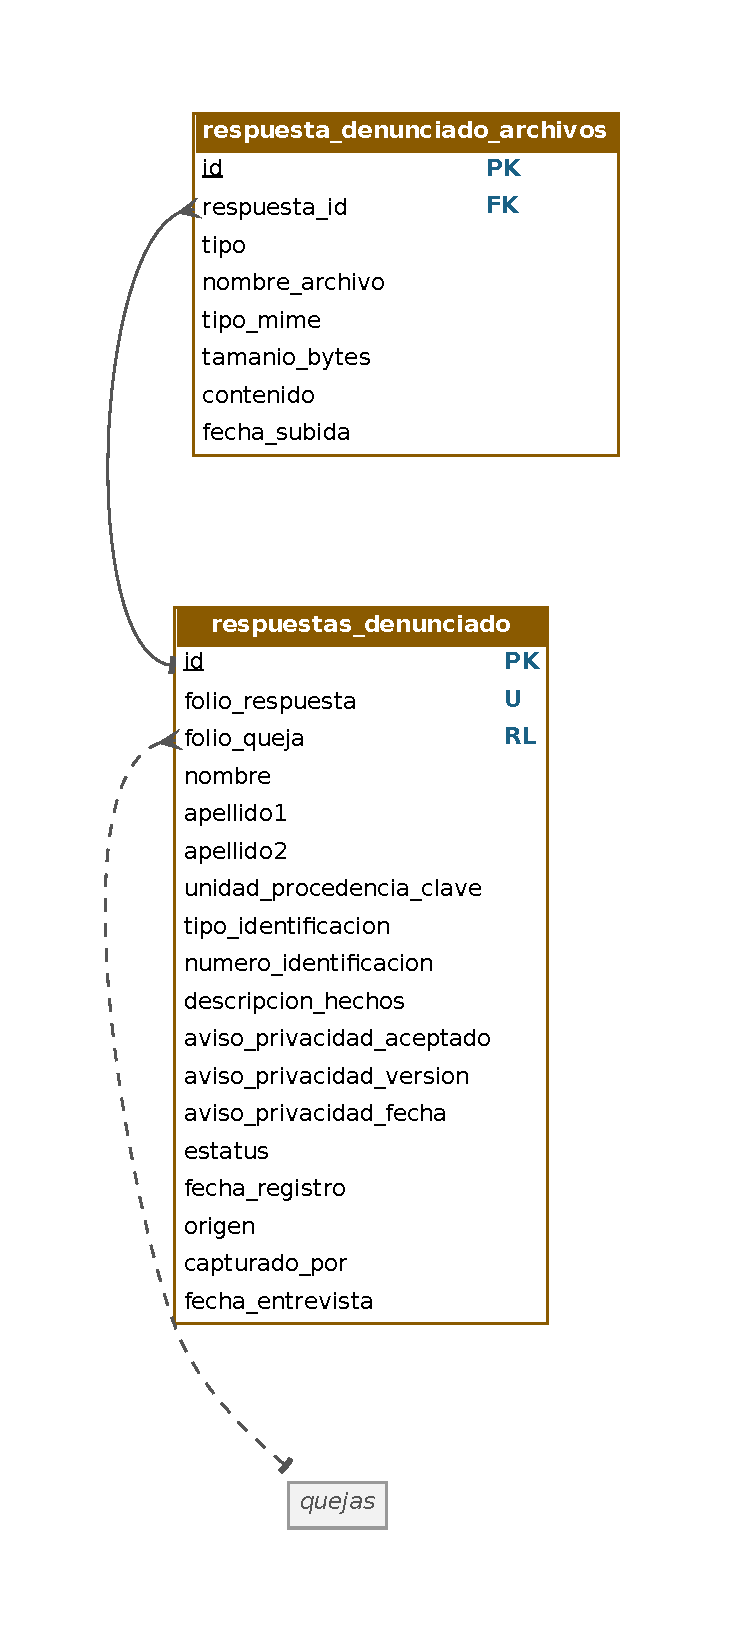
\includegraphics[width=\textwidth,height=0.85\textheight,keepaspectratio]{images/er_grupo_07.pdf}
	\caption{Diagrama entidad-relación: \texttt{respuestas\_denunciado}, \texttt{respuesta\_denunciado\_archivos}}
	\label{fig:er_grupo_07}
\end{figure}

\subsection{Tabla \texttt{respuesta\_denunciado\_archivos}}
Archivos de evidencia que acompañan la respuesta de la persona señalada. Servicio responsable: denunciado-service.


\rowcolors{2}{rowblue}{white}
\footnotesize
\renewcommand{\arraystretch}{1.15}
\setlength{\tabcolsep}{4pt}
\begin{longtable}{|L{3.9cm}|L{2.4cm}|L{0.9cm}|L{1.2cm}|L{6.6cm}|}
	\hiderowcolors\caption{Diccionario de datos de la tabla \texttt{respuesta\_denunciado\_archivos}}
	\label{tab:dic_respuesta_denunciado_archivos} \\ \showrowcolors
	\hline
	\rowcolor{headerblue}
	\headercell{Columna} & \headercell{Tipo} & \headercell{Nulo} & \headercell{Clave} & \headercell{Descripción} \\
	\hline
	\endfirsthead
	\hline
	\rowcolor{headerblue}
	\headercell{Columna} & \headercell{Tipo} & \headercell{Nulo} & \headercell{Clave} & \headercell{Descripción} \\
	\hline
	\endhead
		\texttt{id} & BIGINT & No & PK & Identificador único del registro, generado automáticamente. \\ \hline
		\texttt{respuesta\_\allowbreak{}id} & BIGINT & No & FK & Respuesta a la que pertenece el archivo. \\ \hline
		\texttt{tipo} & VARCHAR(20) & No &  & Clasificación del archivo. \\ \hline
		\texttt{nombre\_\allowbreak{}archivo} & VARCHAR(255) & No &  & Nombre original del archivo. \\ \hline
		\texttt{tipo\_\allowbreak{}mime} & VARCHAR(100) & No &  & Tipo MIME del archivo. \\ \hline
		\texttt{tamanio\_\allowbreak{}bytes} & BIGINT & No &  & Tamaño del archivo en bytes. \\ \hline
		\texttt{contenido} & BYTEA & No &  & Contenido binario del archivo. \\ \hline
		\texttt{fecha\_\allowbreak{}subida} & TIMESTAMP & No &  & Fecha y hora en que se subió el archivo. \\ \hline
\end{longtable}
\normalsize
\setlength{\tabcolsep}{6pt}
\renewcommand{\arraystretch}{1}

\subsection{Tabla \texttt{respuestas\_denunciado}}
Versión de los hechos rendida por la persona señalada, ya sea capturada por ella misma o registrada por el analista. Servicio responsable: denunciado-service.


\rowcolors{2}{rowblue}{white}
\footnotesize
\renewcommand{\arraystretch}{1.15}
\setlength{\tabcolsep}{4pt}
\begin{longtable}{|L{3.9cm}|L{2.4cm}|L{0.9cm}|L{1.2cm}|L{6.6cm}|}
	\hiderowcolors\caption{Diccionario de datos de la tabla \texttt{respuestas\_denunciado}}
	\label{tab:dic_respuestas_denunciado} \\ \showrowcolors
	\hline
	\rowcolor{headerblue}
	\headercell{Columna} & \headercell{Tipo} & \headercell{Nulo} & \headercell{Clave} & \headercell{Descripción} \\
	\hline
	\endfirsthead
	\hline
	\rowcolor{headerblue}
	\headercell{Columna} & \headercell{Tipo} & \headercell{Nulo} & \headercell{Clave} & \headercell{Descripción} \\
	\hline
	\endhead
		\texttt{id} & BIGINT & No & PK & Identificador único del registro, generado automáticamente. \\ \hline
		\texttt{folio\_\allowbreak{}respuesta} & VARCHAR(20) & No & U & Folio único de la respuesta. \\ \hline
		\texttt{folio\_\allowbreak{}queja} & VARCHAR(20) & No & RL & Folio de la queja original. \\ \hline
		\texttt{nombre} & VARCHAR(50) & No &  & Nombre de la persona señalada. \\ \hline
		\texttt{apellido1} & VARCHAR(50) & No &  & Primer apellido de la persona señalada. \\ \hline
		\texttt{apellido2} & VARCHAR(50) & Sí &  & Segundo apellido de la persona señalada. \\ \hline
		\texttt{unidad\_\allowbreak{}procedencia\_\allowbreak{}clave} & VARCHAR(40) & No &  & Clave de la unidad de procedencia de la persona señalada. \\ \hline
		\texttt{tipo\_\allowbreak{}identificacion} & VARCHAR(20) & No &  & Tipo de identificación (boleta o número de empleado). \\ \hline
		\texttt{numero\_\allowbreak{}identificacion} & VARCHAR(10) & No &  & Número de identificación (boleta o número de empleado). \\ \hline
		\texttt{descripcion\_\allowbreak{}hechos} & TEXT & No &  & Versión de los hechos de la persona señalada. \\ \hline
		\texttt{aviso\_\allowbreak{}privacidad\_\allowbreak{}aceptado} & BOOLEAN & No &  & Indica si se aceptó el aviso de privacidad. \\ \hline
		\texttt{aviso\_\allowbreak{}privacidad\_\allowbreak{}version} & VARCHAR(10) & Sí &  & Versión del aviso de privacidad aceptada. \\ \hline
		\texttt{aviso\_\allowbreak{}privacidad\_\allowbreak{}fecha} & TIMESTAMP & Sí &  & Fecha y hora de aceptación del aviso de privacidad. \\ \hline
		\texttt{estatus} & VARCHAR(20) & No &  & Estado de la respuesta. \\ \hline
		\texttt{fecha\_\allowbreak{}registro} & TIMESTAMP & No &  & Fecha y hora del registro. \\ \hline
		\texttt{origen} & VARCHAR(20) & Sí &  & Quién capturó la respuesta (la persona señalada o el analista). \\ \hline
		\texttt{capturado\_\allowbreak{}por} & VARCHAR(120) & Sí &  & Analista que capturó la respuesta, si aplica. \\ \hline
		\texttt{fecha\_\allowbreak{}entrevista} & DATE & Sí &  & Fecha de la entrevista con la persona señalada. \\ \hline
\end{longtable}
\normalsize
\setlength{\tabcolsep}{6pt}
\renewcommand{\arraystretch}{1}

\section{Módulo: Subdefensoría}
\label{anx:bd_mod4}

Las figuras de esta sección muestran el diagrama entidad-relación del módulo con todas sus columnas, divididas en grupos de tablas para facilitar su lectura. Las tablas en gris pertenecen a otros grupos o módulos y se incluyen solo para mostrar las relaciones.


\begin{figure}[H]
	\centering
	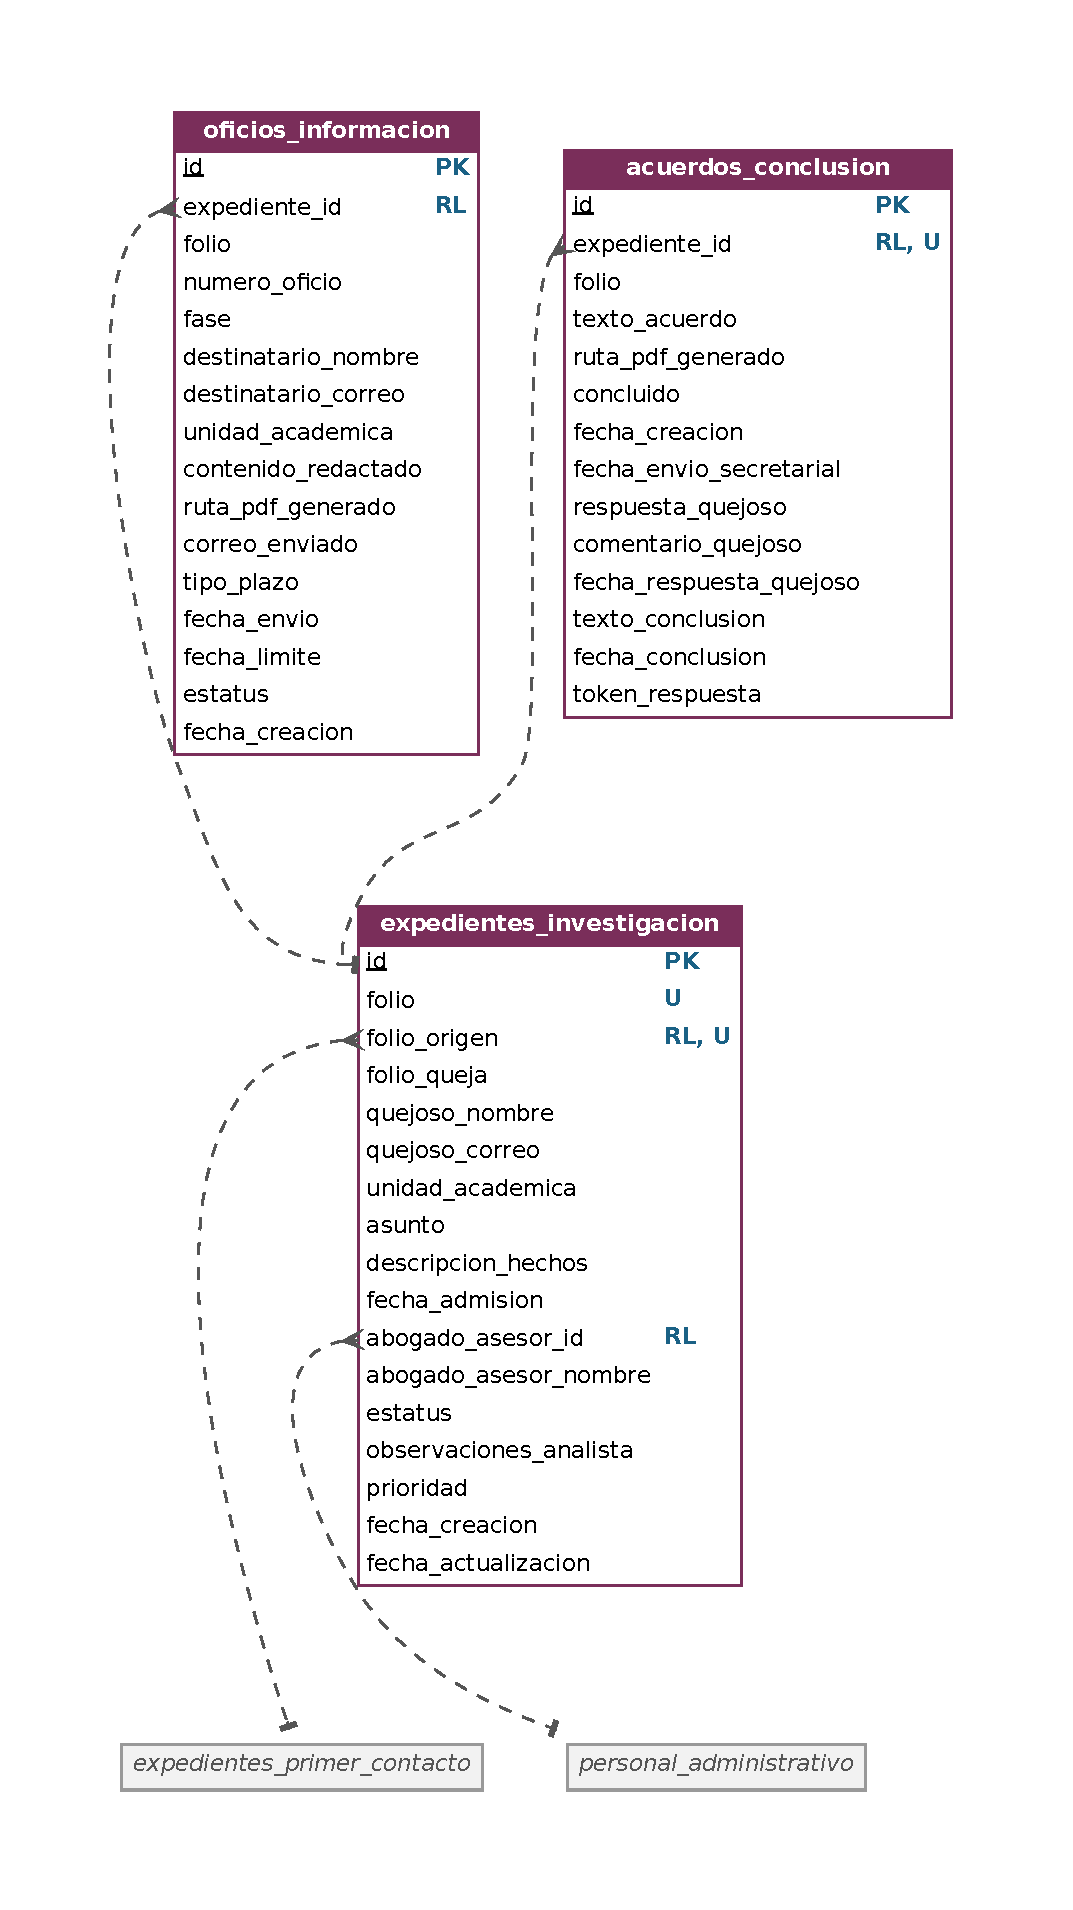
\includegraphics[width=\textwidth,height=0.85\textheight,keepaspectratio]{images/er_grupo_08.pdf}
	\caption{Diagrama entidad-relación: \texttt{expedientes\_investigacion}, \texttt{oficios\_informacion}, \texttt{acuerdos\_conclusion}}
	\label{fig:er_grupo_08}
\end{figure}


\begin{figure}[H]
	\centering
	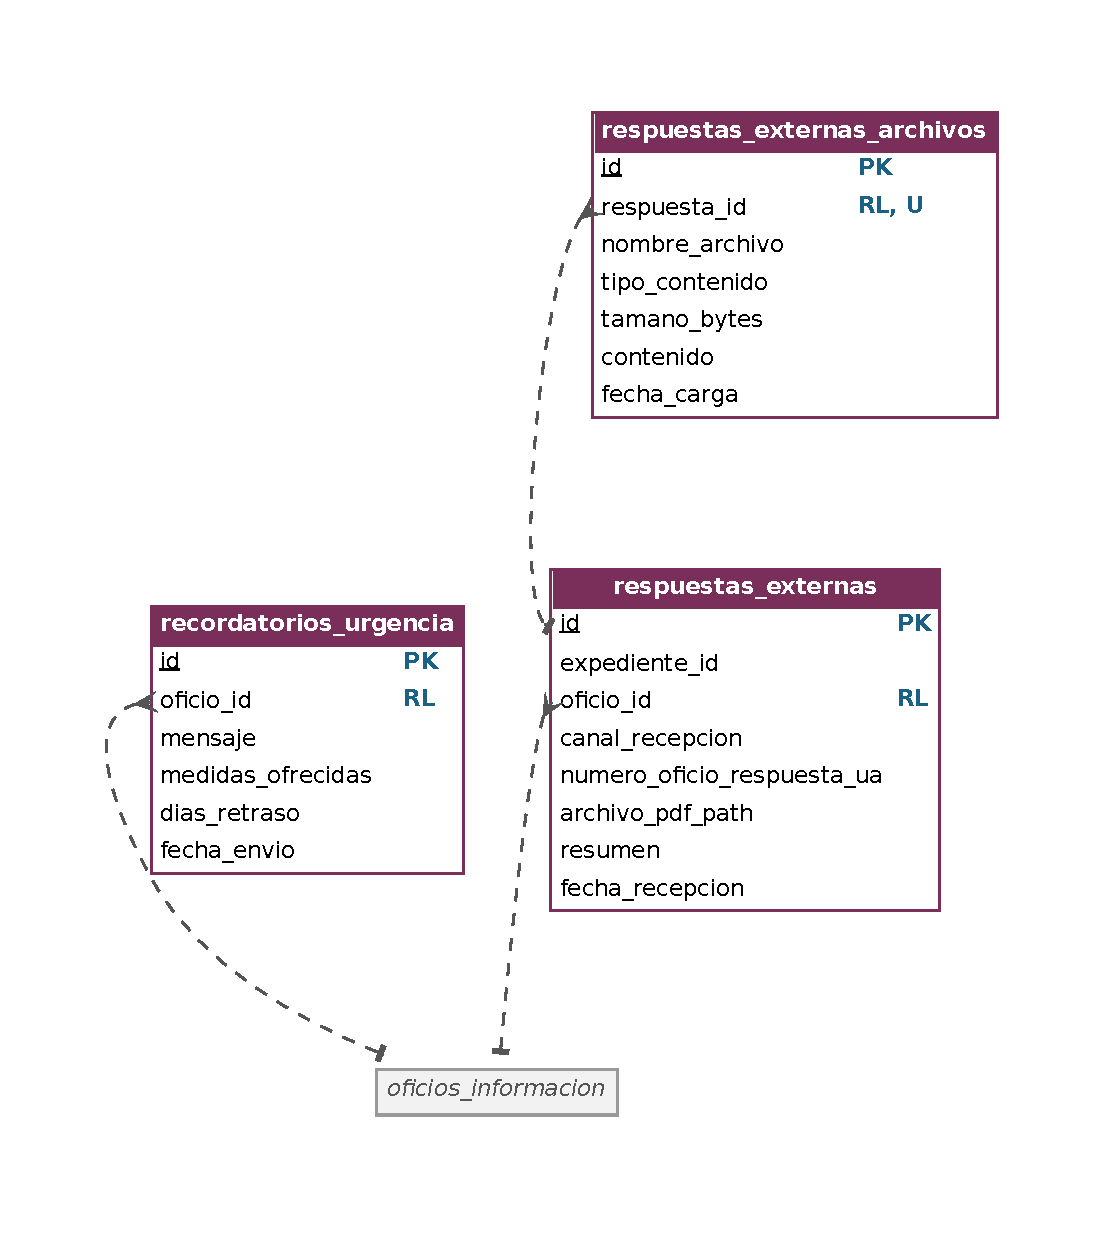
\includegraphics[width=\textwidth,height=0.85\textheight,keepaspectratio]{images/er_grupo_09.pdf}
	\caption{Diagrama entidad-relación: \texttt{recordatorios\_urgencia}, \texttt{respuestas\_externas}, \texttt{respuestas\_externas\_archivos}}
	\label{fig:er_grupo_09}
\end{figure}

\subsection{Tabla \texttt{acuerdos\_conclusion}}
Acuerdo de conciliación y de conclusión con el que se cierra un expediente de investigación, junto con la respuesta del quejoso. Servicio responsable: subdefensoria-service.


\rowcolors{2}{rowblue}{white}
\footnotesize
\renewcommand{\arraystretch}{1.15}
\setlength{\tabcolsep}{4pt}
\begin{longtable}{|L{3.9cm}|L{2.4cm}|L{0.9cm}|L{1.2cm}|L{6.6cm}|}
	\hiderowcolors\caption{Diccionario de datos de la tabla \texttt{acuerdos\_conclusion}}
	\label{tab:dic_acuerdos_conclusion} \\ \showrowcolors
	\hline
	\rowcolor{headerblue}
	\headercell{Columna} & \headercell{Tipo} & \headercell{Nulo} & \headercell{Clave} & \headercell{Descripción} \\
	\hline
	\endfirsthead
	\hline
	\rowcolor{headerblue}
	\headercell{Columna} & \headercell{Tipo} & \headercell{Nulo} & \headercell{Clave} & \headercell{Descripción} \\
	\hline
	\endhead
		\texttt{id} & BIGINT & No & PK & Identificador único del registro, generado automáticamente. \\ \hline
		\texttt{expediente\_\allowbreak{}id} & BIGINT & No & RL, U & Expediente al que pertenece el registro. \\ \hline
		\texttt{folio} & VARCHAR(50) & No &  & Folio del expediente de investigación. \\ \hline
		\texttt{texto\_\allowbreak{}acuerdo} & TEXT & No &  & Texto del acuerdo de conciliación. \\ \hline
		\texttt{ruta\_\allowbreak{}pdf\_\allowbreak{}generado} & VARCHAR(300) & Sí &  & Ruta del PDF generado. \\ \hline
		\texttt{concluido} & BOOLEAN & No &  & Indica si el expediente quedó concluido. \\ \hline
		\texttt{fecha\_\allowbreak{}creacion} & TIMESTAMP & No &  & Fecha y hora de creación del registro. \\ \hline
		\texttt{fecha\_\allowbreak{}envio\_\allowbreak{}secretarial} & TIMESTAMP & Sí &  & Fecha de envío del acuerdo para firma. \\ \hline
		\texttt{respuesta\_\allowbreak{}quejoso} & VARCHAR(20) & Sí &  & Respuesta del quejoso al acuerdo (acepta o rechaza). \\ \hline
		\texttt{comentario\_\allowbreak{}quejoso} & TEXT & Sí &  & Comentario del quejoso al responder. \\ \hline
		\texttt{fecha\_\allowbreak{}respuesta\_\allowbreak{}quejoso} & TIMESTAMP & Sí &  & Fecha y hora de la respuesta del quejoso. \\ \hline
		\texttt{texto\_\allowbreak{}conclusion} & TEXT & Sí &  & Texto del acuerdo de conclusión. \\ \hline
		\texttt{fecha\_\allowbreak{}conclusion} & TIMESTAMP & Sí &  & Fecha de conclusión del expediente. \\ \hline
		\texttt{token\_\allowbreak{}respuesta} & VARCHAR(64) & Sí &  & Token del enlace con el que la persona responde sin iniciar sesión. \\ \hline
\end{longtable}
\normalsize
\setlength{\tabcolsep}{6pt}
\renewcommand{\arraystretch}{1}

\subsection{Tabla \texttt{expedientes\_investigacion}}
Expediente de investigación que se crea cuando Primer Contacto dictamina una queja como procedente; registra el abogado asignado, la etapa y la prioridad. Servicio responsable: subdefensoria-service.


\rowcolors{2}{rowblue}{white}
\footnotesize
\renewcommand{\arraystretch}{1.15}
\setlength{\tabcolsep}{4pt}
\begin{longtable}{|L{3.9cm}|L{2.4cm}|L{0.9cm}|L{1.2cm}|L{6.6cm}|}
	\hiderowcolors\caption{Diccionario de datos de la tabla \texttt{expedientes\_investigacion}}
	\label{tab:dic_expedientes_investigacion} \\ \showrowcolors
	\hline
	\rowcolor{headerblue}
	\headercell{Columna} & \headercell{Tipo} & \headercell{Nulo} & \headercell{Clave} & \headercell{Descripción} \\
	\hline
	\endfirsthead
	\hline
	\rowcolor{headerblue}
	\headercell{Columna} & \headercell{Tipo} & \headercell{Nulo} & \headercell{Clave} & \headercell{Descripción} \\
	\hline
	\endhead
		\texttt{id} & BIGINT & No & PK & Identificador único del registro, generado automáticamente. \\ \hline
		\texttt{folio} & VARCHAR(50) & No & U & Folio del expediente en Subdefensoría. \\ \hline
		\texttt{folio\_\allowbreak{}origen} & VARCHAR(50) & No & RL, U & Folio del expediente en Primer Contacto. \\ \hline
		\texttt{folio\_\allowbreak{}queja} & VARCHAR(50) & Sí &  & Folio de la queja original. \\ \hline
		\texttt{quejoso\_\allowbreak{}nombre} & VARCHAR(150) & Sí &  & Nombre del quejoso. \\ \hline
		\texttt{quejoso\_\allowbreak{}correo} & VARCHAR(150) & Sí &  & Correo electrónico del quejoso. \\ \hline
		\texttt{unidad\_\allowbreak{}academica} & VARCHAR(100) & Sí &  & Unidad académica relacionada. \\ \hline
		\texttt{asunto} & VARCHAR(200) & Sí &  & Asunto o tema del documento. \\ \hline
		\texttt{descripcion\_\allowbreak{}hechos} & TEXT & Sí &  & Narrativa de los hechos de la queja. \\ \hline
		\texttt{fecha\_\allowbreak{}admision} & DATE & No &  & Fecha en que el expediente se admitió en Subdefensoría. \\ \hline
		\texttt{abogado\_\allowbreak{}asesor\_\allowbreak{}id} & BIGINT & Sí & RL & Identificador del abogado de Subdefensoría asignado (personal administrativo). \\ \hline
		\texttt{abogado\_\allowbreak{}asesor\_\allowbreak{}nombre} & VARCHAR(150) & Sí &  & Nombre del abogado asignado, conservado para consulta. \\ \hline
		\texttt{estatus} & VARCHAR(30) & No &  & Etapa de la investigación (RECIBIDO, EN\_INVESTIGACION, EN\_ESPERA\_OFICIO, CONCLUIDO, entre otras). \\ \hline
		\texttt{observaciones\_\allowbreak{}analista} & TEXT & Sí &  & Observaciones del analista de Primer Contacto al turnar. \\ \hline
		\texttt{prioridad} & VARCHAR(10) & Sí &  & Prioridad del expediente (baja, media, alta o urgente). \\ \hline
		\texttt{fecha\_\allowbreak{}creacion} & TIMESTAMP & No &  & Fecha y hora de creación del registro. \\ \hline
		\texttt{fecha\_\allowbreak{}actualizacion} & TIMESTAMP & Sí &  & Fecha y hora de la última actualización. \\ \hline
\end{longtable}
\normalsize
\setlength{\tabcolsep}{6pt}
\renewcommand{\arraystretch}{1}

\subsection{Tabla \texttt{oficios\_informacion}}
Oficios de solicitud de información enviados a las unidades, con su plazo y fecha límite. Servicio responsable: subdefensoria-service.


\rowcolors{2}{rowblue}{white}
\footnotesize
\renewcommand{\arraystretch}{1.15}
\setlength{\tabcolsep}{4pt}
\begin{longtable}{|L{3.9cm}|L{2.4cm}|L{0.9cm}|L{1.2cm}|L{6.6cm}|}
	\hiderowcolors\caption{Diccionario de datos de la tabla \texttt{oficios\_informacion}}
	\label{tab:dic_oficios_informacion} \\ \showrowcolors
	\hline
	\rowcolor{headerblue}
	\headercell{Columna} & \headercell{Tipo} & \headercell{Nulo} & \headercell{Clave} & \headercell{Descripción} \\
	\hline
	\endfirsthead
	\hline
	\rowcolor{headerblue}
	\headercell{Columna} & \headercell{Tipo} & \headercell{Nulo} & \headercell{Clave} & \headercell{Descripción} \\
	\hline
	\endhead
		\texttt{id} & BIGINT & No & PK & Identificador único del registro, generado automáticamente. \\ \hline
		\texttt{expediente\_\allowbreak{}id} & BIGINT & No & RL & Expediente al que pertenece el registro. \\ \hline
		\texttt{folio} & VARCHAR(50) & No &  & Folio del expediente de investigación. \\ \hline
		\texttt{numero\_\allowbreak{}oficio} & VARCHAR(50) & No &  & Número del oficio. \\ \hline
		\texttt{fase} & VARCHAR(30) & No &  & Fase del oficio (primera solicitud o recordatorio). \\ \hline
		\texttt{destinatario\_\allowbreak{}nombre} & VARCHAR(200) & No &  & Nombre del titular de la unidad destinataria. \\ \hline
		\texttt{destinatario\_\allowbreak{}correo} & VARCHAR(150) & No &  & Correo electrónico del titular de la unidad destinataria. \\ \hline
		\texttt{unidad\_\allowbreak{}academica} & VARCHAR(100) & Sí &  & Unidad académica relacionada. \\ \hline
		\texttt{contenido\_\allowbreak{}redactado} & TEXT & No &  & Texto del oficio redactado. \\ \hline
		\texttt{ruta\_\allowbreak{}pdf\_\allowbreak{}generado} & VARCHAR(300) & Sí &  & Ruta del PDF generado. \\ \hline
		\texttt{correo\_\allowbreak{}enviado} & BOOLEAN & Sí &  & Indica si el correo se envió correctamente. \\ \hline
		\texttt{tipo\_\allowbreak{}plazo} & VARCHAR(20) & No &  & Plazo aplicable al oficio (diez o cinco días hábiles). \\ \hline
		\texttt{fecha\_\allowbreak{}envio} & DATE & No &  & Fecha de envío. \\ \hline
		\texttt{fecha\_\allowbreak{}limite} & DATE & No &  & Fecha límite de respuesta según el plazo aplicable. \\ \hline
		\texttt{estatus} & VARCHAR(20) & No &  & Estado del oficio. \\ \hline
		\texttt{fecha\_\allowbreak{}creacion} & TIMESTAMP & No &  & Fecha y hora de creación del registro. \\ \hline
\end{longtable}
\normalsize
\setlength{\tabcolsep}{6pt}
\renewcommand{\arraystretch}{1}

\subsection{Tabla \texttt{recordatorios\_urgencia}}
Recordatorios enviados cuando una unidad no responde un oficio dentro del plazo. Servicio responsable: subdefensoria-service.


\rowcolors{2}{rowblue}{white}
\footnotesize
\renewcommand{\arraystretch}{1.15}
\setlength{\tabcolsep}{4pt}
\begin{longtable}{|L{3.9cm}|L{2.4cm}|L{0.9cm}|L{1.2cm}|L{6.6cm}|}
	\hiderowcolors\caption{Diccionario de datos de la tabla \texttt{recordatorios\_urgencia}}
	\label{tab:dic_recordatorios_urgencia} \\ \showrowcolors
	\hline
	\rowcolor{headerblue}
	\headercell{Columna} & \headercell{Tipo} & \headercell{Nulo} & \headercell{Clave} & \headercell{Descripción} \\
	\hline
	\endfirsthead
	\hline
	\rowcolor{headerblue}
	\headercell{Columna} & \headercell{Tipo} & \headercell{Nulo} & \headercell{Clave} & \headercell{Descripción} \\
	\hline
	\endhead
		\texttt{id} & BIGINT & No & PK & Identificador único del registro, generado automáticamente. \\ \hline
		\texttt{oficio\_\allowbreak{}id} & BIGINT & No & RL & Oficio al que corresponde el registro. \\ \hline
		\texttt{mensaje} & TEXT & No &  & Texto del mensaje. \\ \hline
		\texttt{medidas\_\allowbreak{}ofrecidas} & TEXT & Sí &  & Medidas ofrecidas a la unidad en el recordatorio. \\ \hline
		\texttt{dias\_\allowbreak{}retraso} & INTEGER & No &  & Días transcurridos desde el vencimiento del plazo. \\ \hline
		\texttt{fecha\_\allowbreak{}envio} & TIMESTAMP & No &  & Fecha de envío. \\ \hline
\end{longtable}
\normalsize
\setlength{\tabcolsep}{6pt}
\renewcommand{\arraystretch}{1}

\subsection{Tabla \texttt{respuestas\_externas}}
Respuestas recibidas de las unidades a los oficios de solicitud de información. Servicio responsable: subdefensoria-service.


\rowcolors{2}{rowblue}{white}
\footnotesize
\renewcommand{\arraystretch}{1.15}
\setlength{\tabcolsep}{4pt}
\begin{longtable}{|L{3.9cm}|L{2.4cm}|L{0.9cm}|L{1.2cm}|L{6.6cm}|}
	\hiderowcolors\caption{Diccionario de datos de la tabla \texttt{respuestas\_externas}}
	\label{tab:dic_respuestas_externas} \\ \showrowcolors
	\hline
	\rowcolor{headerblue}
	\headercell{Columna} & \headercell{Tipo} & \headercell{Nulo} & \headercell{Clave} & \headercell{Descripción} \\
	\hline
	\endfirsthead
	\hline
	\rowcolor{headerblue}
	\headercell{Columna} & \headercell{Tipo} & \headercell{Nulo} & \headercell{Clave} & \headercell{Descripción} \\
	\hline
	\endhead
		\texttt{id} & BIGINT & No & PK & Identificador único del registro, generado automáticamente. \\ \hline
		\texttt{expediente\_\allowbreak{}id} & BIGINT & No &  & Expediente al que pertenece el registro. \\ \hline
		\texttt{oficio\_\allowbreak{}id} & BIGINT & No & RL & Oficio al que corresponde el registro. \\ \hline
		\texttt{canal\_\allowbreak{}recepcion} & VARCHAR(100) & No &  & Medio por el que se recibió la respuesta (correo, oficio físico, etc.). \\ \hline
		\texttt{numero\_\allowbreak{}oficio\_\allowbreak{}respuesta\_\allowbreak{}ua} & VARCHAR(100) & Sí &  & Número del oficio con el que respondió la unidad. \\ \hline
		\texttt{archivo\_\allowbreak{}pdf\_\allowbreak{}path} & VARCHAR(300) & Sí &  & Ruta del archivo PDF de la respuesta. \\ \hline
		\texttt{resumen} & TEXT & No &  & Texto del resumen. \\ \hline
		\texttt{fecha\_\allowbreak{}recepcion} & TIMESTAMP & No &  & Fecha y hora de recepción. \\ \hline
\end{longtable}
\normalsize
\setlength{\tabcolsep}{6pt}
\renewcommand{\arraystretch}{1}

\subsection{Tabla \texttt{respuestas\_externas\_archivos}}
Archivo digital asociado a la respuesta de una unidad. Servicio responsable: subdefensoria-service.


\rowcolors{2}{rowblue}{white}
\footnotesize
\renewcommand{\arraystretch}{1.15}
\setlength{\tabcolsep}{4pt}
\begin{longtable}{|L{3.9cm}|L{2.4cm}|L{0.9cm}|L{1.2cm}|L{6.6cm}|}
	\hiderowcolors\caption{Diccionario de datos de la tabla \texttt{respuestas\_externas\_archivos}}
	\label{tab:dic_respuestas_externas_archivos} \\ \showrowcolors
	\hline
	\rowcolor{headerblue}
	\headercell{Columna} & \headercell{Tipo} & \headercell{Nulo} & \headercell{Clave} & \headercell{Descripción} \\
	\hline
	\endfirsthead
	\hline
	\rowcolor{headerblue}
	\headercell{Columna} & \headercell{Tipo} & \headercell{Nulo} & \headercell{Clave} & \headercell{Descripción} \\
	\hline
	\endhead
		\texttt{id} & BIGINT & No & PK & Identificador único del registro, generado automáticamente. \\ \hline
		\texttt{respuesta\_\allowbreak{}id} & BIGINT & No & RL, U & Respuesta a la que pertenece el archivo. \\ \hline
		\texttt{nombre\_\allowbreak{}archivo} & VARCHAR(255) & No &  & Nombre original del archivo. \\ \hline
		\texttt{tipo\_\allowbreak{}contenido} & VARCHAR(50) & No &  & Tipo MIME del archivo. \\ \hline
		\texttt{tamano\_\allowbreak{}bytes} & BIGINT & No &  & Tamaño del archivo en bytes. \\ \hline
		\texttt{contenido} & BYTEA & No &  & Contenido binario del archivo. \\ \hline
		\texttt{fecha\_\allowbreak{}carga} & TIMESTAMP & No &  & Fecha de carga del archivo. \\ \hline
\end{longtable}
\normalsize
\setlength{\tabcolsep}{6pt}
\renewcommand{\arraystretch}{1}

\section{Módulo: Administración y catálogos}
\label{anx:bd_mod5}

Las figuras de esta sección muestran el diagrama entidad-relación del módulo con todas sus columnas, divididas en grupos de tablas para facilitar su lectura. Las tablas en gris pertenecen a otros grupos o módulos y se incluyen solo para mostrar las relaciones.


\begin{figure}[H]
	\centering
	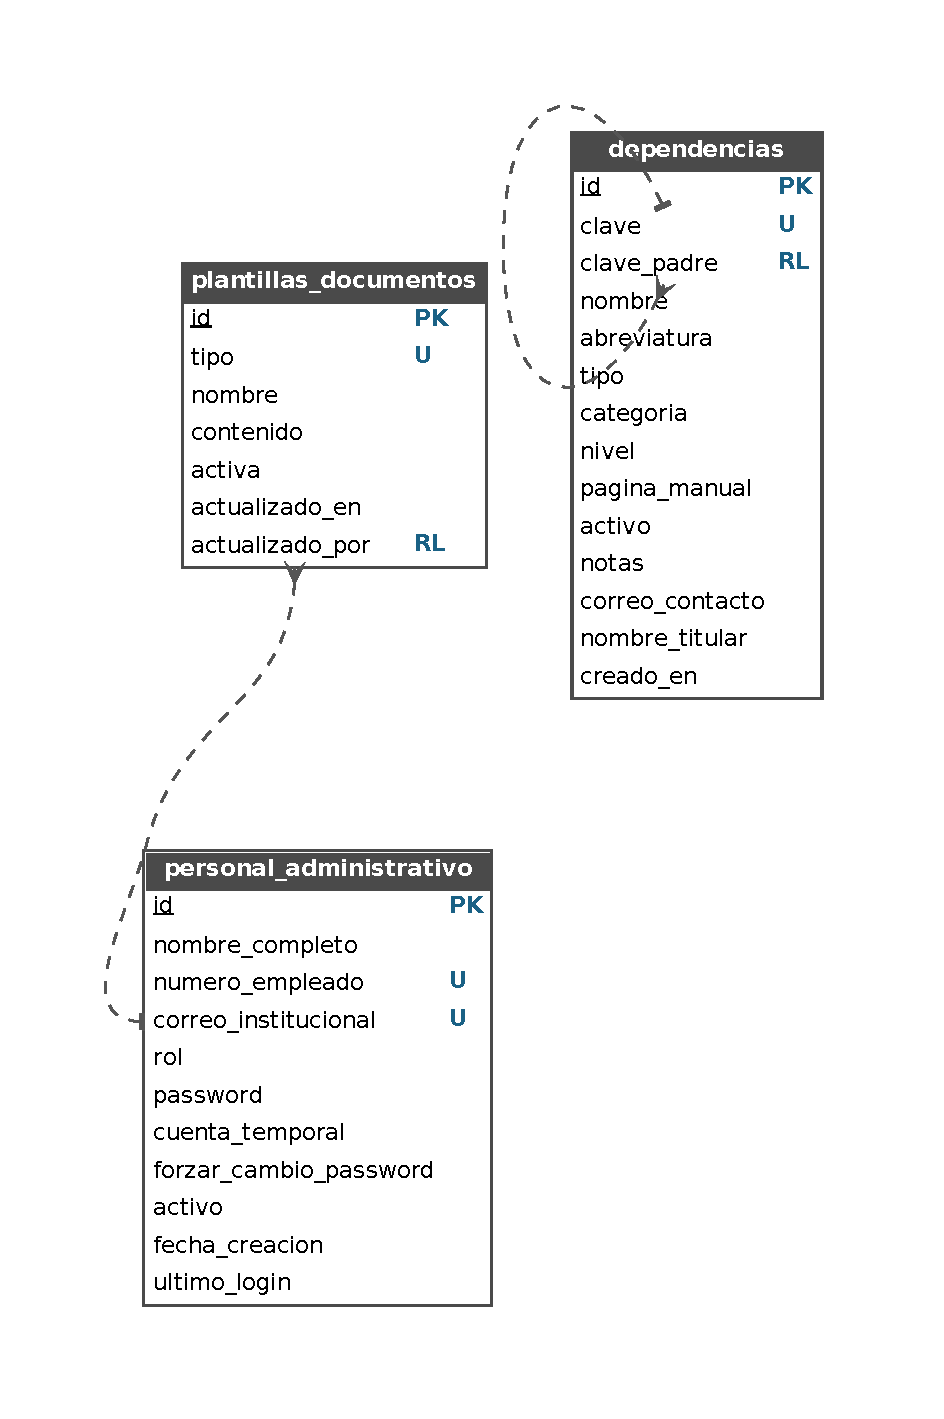
\includegraphics[width=\textwidth,height=0.85\textheight,keepaspectratio]{images/er_grupo_10.pdf}
	\caption{Diagrama entidad-relación: \texttt{personal\_administrativo}, \texttt{dependencias}, \texttt{plantillas\_documentos}}
	\label{fig:er_grupo_10}
\end{figure}


\begin{figure}[H]
	\centering
	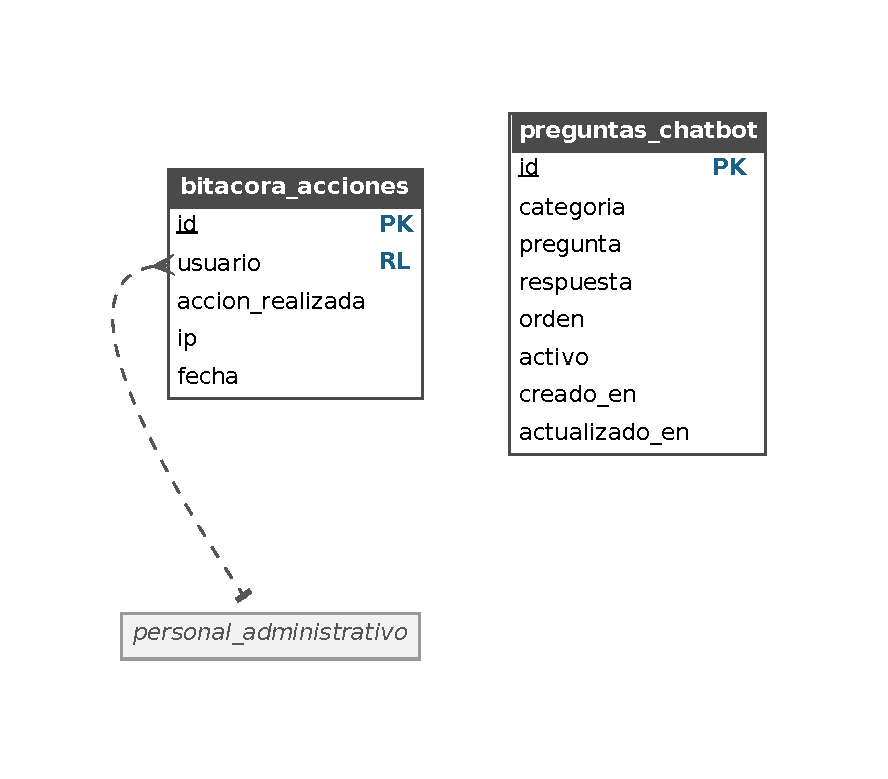
\includegraphics[width=\textwidth,height=0.85\textheight,keepaspectratio]{images/er_grupo_11.pdf}
	\caption{Diagrama entidad-relación: \texttt{bitacora\_acciones}, \texttt{preguntas\_chatbot}}
	\label{fig:er_grupo_11}
\end{figure}

\subsection{Tabla \texttt{bitacora\_acciones}}
Bitácora de auditoría de las acciones administrativas: usuario, acción, dirección de origen y fecha. Servicio responsable: admin-service.


\rowcolors{2}{rowblue}{white}
\footnotesize
\renewcommand{\arraystretch}{1.15}
\setlength{\tabcolsep}{4pt}
\begin{longtable}{|L{3.9cm}|L{2.4cm}|L{0.9cm}|L{1.2cm}|L{6.6cm}|}
	\hiderowcolors\caption{Diccionario de datos de la tabla \texttt{bitacora\_acciones}}
	\label{tab:dic_bitacora_acciones} \\ \showrowcolors
	\hline
	\rowcolor{headerblue}
	\headercell{Columna} & \headercell{Tipo} & \headercell{Nulo} & \headercell{Clave} & \headercell{Descripción} \\
	\hline
	\endfirsthead
	\hline
	\rowcolor{headerblue}
	\headercell{Columna} & \headercell{Tipo} & \headercell{Nulo} & \headercell{Clave} & \headercell{Descripción} \\
	\hline
	\endhead
		\texttt{id} & BIGINT & No & PK & Identificador único del registro, generado automáticamente. \\ \hline
		\texttt{usuario} & VARCHAR(255) & No & RL & Usuario que realizó la acción. \\ \hline
		\texttt{accion\_\allowbreak{}realizada} & VARCHAR(255) & No &  & Descripción de la acción administrativa realizada. \\ \hline
		\texttt{ip} & VARCHAR(255) & No &  & Dirección IP de origen de la acción. \\ \hline
		\texttt{fecha} & TIMESTAMP & No &  & Fecha y hora de la acción. \\ \hline
\end{longtable}
\normalsize
\setlength{\tabcolsep}{6pt}
\renewcommand{\arraystretch}{1}

\subsection{Tabla \texttt{dependencias}}
Catálogo jerárquico de dependencias y unidades académicas del Instituto, con su titular y correo de contacto. Servicio responsable: catalogo-service.


\rowcolors{2}{rowblue}{white}
\footnotesize
\renewcommand{\arraystretch}{1.15}
\setlength{\tabcolsep}{4pt}
\begin{longtable}{|L{3.9cm}|L{2.4cm}|L{0.9cm}|L{1.2cm}|L{6.6cm}|}
	\hiderowcolors\caption{Diccionario de datos de la tabla \texttt{dependencias}}
	\label{tab:dic_dependencias} \\ \showrowcolors
	\hline
	\rowcolor{headerblue}
	\headercell{Columna} & \headercell{Tipo} & \headercell{Nulo} & \headercell{Clave} & \headercell{Descripción} \\
	\hline
	\endfirsthead
	\hline
	\rowcolor{headerblue}
	\headercell{Columna} & \headercell{Tipo} & \headercell{Nulo} & \headercell{Clave} & \headercell{Descripción} \\
	\hline
	\endhead
		\texttt{id} & BIGINT & No & PK & Identificador único del registro, generado automáticamente. \\ \hline
		\texttt{clave} & VARCHAR(20) & No & U & Clave única de la dependencia. \\ \hline
		\texttt{clave\_\allowbreak{}padre} & VARCHAR(20) & Sí & RL & Clave de la dependencia superior en la jerarquía. \\ \hline
		\texttt{nombre} & VARCHAR(255) & No &  & Nombre oficial de la dependencia. \\ \hline
		\texttt{abreviatura} & VARCHAR(30) & Sí &  & Abreviatura o siglas de la dependencia. \\ \hline
		\texttt{tipo} & VARCHAR(60) & No &  & Tipo de dependencia. \\ \hline
		\texttt{categoria} & VARCHAR(150) & Sí &  & Categoría de la dependencia (escuela superior, centro de investigación, etc.). \\ \hline
		\texttt{nivel} & INTEGER & No &  & Nivel jerárquico de la dependencia. \\ \hline
		\texttt{pagina\_\allowbreak{}manual} & INTEGER & Sí &  & Página del manual de organización donde aparece la dependencia. \\ \hline
		\texttt{activo} & BOOLEAN & No &  & Indica si el registro está activo. \\ \hline
		\texttt{notas} & TEXT & Sí &  & Notas adicionales. \\ \hline
		\texttt{correo\_\allowbreak{}contacto} & VARCHAR(150) & Sí &  & Correo electrónico de contacto de la dependencia. \\ \hline
		\texttt{nombre\_\allowbreak{}titular} & VARCHAR(150) & Sí &  & Nombre del titular de la dependencia. \\ \hline
		\texttt{creado\_\allowbreak{}en} & TIMESTAMP & Sí &  & Fecha y hora de creación. \\ \hline
\end{longtable}
\normalsize
\setlength{\tabcolsep}{6pt}
\renewcommand{\arraystretch}{1}

\subsection{Tabla \texttt{personal\_administrativo}}
Cuentas del personal de la Defensoría con su rol, estado de la cuenta y último acceso. Servicio responsable: admin-service, revision-service, primer-contacto-service.


\rowcolors{2}{rowblue}{white}
\footnotesize
\renewcommand{\arraystretch}{1.15}
\setlength{\tabcolsep}{4pt}
\begin{longtable}{|L{3.9cm}|L{2.4cm}|L{0.9cm}|L{1.2cm}|L{6.6cm}|}
	\hiderowcolors\caption{Diccionario de datos de la tabla \texttt{personal\_administrativo}}
	\label{tab:dic_personal_administrativo} \\ \showrowcolors
	\hline
	\rowcolor{headerblue}
	\headercell{Columna} & \headercell{Tipo} & \headercell{Nulo} & \headercell{Clave} & \headercell{Descripción} \\
	\hline
	\endfirsthead
	\hline
	\rowcolor{headerblue}
	\headercell{Columna} & \headercell{Tipo} & \headercell{Nulo} & \headercell{Clave} & \headercell{Descripción} \\
	\hline
	\endhead
		\texttt{id} & BIGINT & No & PK & Identificador único del registro, generado automáticamente. \\ \hline
		\texttt{nombre\_\allowbreak{}completo} & VARCHAR(255) & No &  & Nombre completo de la persona. \\ \hline
		\texttt{numero\_\allowbreak{}empleado} & VARCHAR(255) & No & U & Número de empleado. \\ \hline
		\texttt{correo\_\allowbreak{}institucional} & VARCHAR(255) & No & U & Correo institucional; se usa para iniciar sesión. \\ \hline
		\texttt{rol} & VARCHAR(255) & No &  & Rol del usuario (RECEPCIONISTA, ANALISTA\_PRIMER\_CONTACTO, SUBDEFENSOR o DEFENSOR). \\ \hline
		\texttt{password} & VARCHAR(255) & No &  & Contraseña cifrada mediante función de resumen. \\ \hline
		\texttt{cuenta\_\allowbreak{}temporal} & BOOLEAN & No &  & Indica si la cuenta conserva la contraseña temporal. \\ \hline
		\texttt{forzar\_\allowbreak{}cambio\_\allowbreak{}password} & BOOLEAN & No &  & Indica si el usuario debe cambiar su contraseña en el siguiente inicio de sesión. \\ \hline
		\texttt{activo} & BOOLEAN & No &  & Indica si la cuenta está activa; dar de baja la desactiva sin eliminarla. \\ \hline
		\texttt{fecha\_\allowbreak{}creacion} & TIMESTAMP & No &  & Fecha y hora de creación del registro. \\ \hline
		\texttt{ultimo\_\allowbreak{}login} & TIMESTAMP & Sí &  & Fecha y hora del último inicio de sesión. \\ \hline
\end{longtable}
\normalsize
\setlength{\tabcolsep}{6pt}
\renewcommand{\arraystretch}{1}

\subsection{Tabla \texttt{plantillas\_documentos}}
Plantillas de los oficios y documentos que genera la plataforma. Servicio responsable: admin-service.


\rowcolors{2}{rowblue}{white}
\footnotesize
\renewcommand{\arraystretch}{1.15}
\setlength{\tabcolsep}{4pt}
\begin{longtable}{|L{3.9cm}|L{2.4cm}|L{0.9cm}|L{1.2cm}|L{6.6cm}|}
	\hiderowcolors\caption{Diccionario de datos de la tabla \texttt{plantillas\_documentos}}
	\label{tab:dic_plantillas_documentos} \\ \showrowcolors
	\hline
	\rowcolor{headerblue}
	\headercell{Columna} & \headercell{Tipo} & \headercell{Nulo} & \headercell{Clave} & \headercell{Descripción} \\
	\hline
	\endfirsthead
	\hline
	\rowcolor{headerblue}
	\headercell{Columna} & \headercell{Tipo} & \headercell{Nulo} & \headercell{Clave} & \headercell{Descripción} \\
	\hline
	\endhead
		\texttt{id} & BIGINT & No & PK & Identificador único del registro, generado automáticamente. \\ \hline
		\texttt{tipo} & VARCHAR(80) & No & U & Clave estable de la plantilla. \\ \hline
		\texttt{nombre} & VARCHAR(255) & No &  & Nombre descriptivo de la plantilla. \\ \hline
		\texttt{contenido} & TEXT & No &  & Contenido de la plantilla con sus marcadores. \\ \hline
		\texttt{activa} & BOOLEAN & No &  & Indica si la plantilla está vigente. \\ \hline
		\texttt{actualizado\_\allowbreak{}en} & TIMESTAMP & Sí &  & Fecha y hora de la última actualización. \\ \hline
		\texttt{actualizado\_\allowbreak{}por} & VARCHAR(255) & Sí & RL & Usuario que realizó la última actualización. \\ \hline
\end{longtable}
\normalsize
\setlength{\tabcolsep}{6pt}
\renewcommand{\arraystretch}{1}

\subsection{Tabla \texttt{preguntas\_chatbot}}
Preguntas y respuestas del menú de ayuda del portal público. Servicio responsable: chatbot-service.


\rowcolors{2}{rowblue}{white}
\footnotesize
\renewcommand{\arraystretch}{1.15}
\setlength{\tabcolsep}{4pt}
\begin{longtable}{|L{3.9cm}|L{2.4cm}|L{0.9cm}|L{1.2cm}|L{6.6cm}|}
	\hiderowcolors\caption{Diccionario de datos de la tabla \texttt{preguntas\_chatbot}}
	\label{tab:dic_preguntas_chatbot} \\ \showrowcolors
	\hline
	\rowcolor{headerblue}
	\headercell{Columna} & \headercell{Tipo} & \headercell{Nulo} & \headercell{Clave} & \headercell{Descripción} \\
	\hline
	\endfirsthead
	\hline
	\rowcolor{headerblue}
	\headercell{Columna} & \headercell{Tipo} & \headercell{Nulo} & \headercell{Clave} & \headercell{Descripción} \\
	\hline
	\endhead
		\texttt{id} & BIGINT & No & PK & Identificador único del registro, generado automáticamente. \\ \hline
		\texttt{categoria} & VARCHAR(80) & No &  & Categoría de la pregunta. \\ \hline
		\texttt{pregunta} & VARCHAR(300) & No &  & Texto de la pregunta. \\ \hline
		\texttt{respuesta} & TEXT & No &  & Texto de la respuesta. \\ \hline
		\texttt{orden} & INTEGER & No &  & Posición de despliegue en las listas. \\ \hline
		\texttt{activo} & BOOLEAN & No &  & Indica si la pregunta se muestra en el portal. \\ \hline
		\texttt{creado\_\allowbreak{}en} & TIMESTAMP & Sí &  & Fecha y hora de creación. \\ \hline
		\texttt{actualizado\_\allowbreak{}en} & TIMESTAMP & Sí &  & Fecha y hora de la última actualización. \\ \hline
\end{longtable}
\normalsize
\setlength{\tabcolsep}{6pt}
\renewcommand{\arraystretch}{1}
